\documentclass[12pt, letterpaper]{article} 
%\documentclass[12pt, letterpaper, doublespace]{article} 
\usepackage[top=1in, bottom=1in, left=1in, right=1in]{geometry} 
\usepackage{setspace}
\doublespacing
\usepackage{amsmath} 
\usepackage{amsfonts} 
\usepackage{natbib}
\usepackage{mathtools} 
\usepackage{ragged2e} % for text justification
\usepackage{adjustbox} 
\usepackage{amssymb}
%\usepackage[capposition=top]{floatrow} 
\usepackage{fullpage} 
\usepackage{listings}
\usepackage{dcolumn} 
\usepackage{bigstrut} 
\usepackage{float} 
\usepackage{enumitem} 
\usepackage{url}
\usepackage[clockwise]{rotating} 
\usepackage{rotfloat} 
\usepackage{rotate} 
\usepackage{rotating}
\usepackage{pdflscape} 
\usepackage[labelfont=bf]{caption} 
\usepackage{graphicx} 
\usepackage{array}
\usepackage{booktabs} 
\usepackage[flushleft]{threeparttable} 
\usepackage{threeparttablex} 
% Lets threeparttable work with longtable 
\usepackage[outdir=graphics/]{epstopdf} 
\usepackage{graphics}
\usepackage{longtable} 
\usepackage[width=.95\textwidth]{caption}
\usepackage{changepage} 
% for the adjustwidth environment
%\let\oldtabular\tabular 
%\renewcommand{\tabular}{\footnotesize\oldtabular}
\newcommand\Fontvi{\fontsize{8}{7.2}\selectfont}
%\newcolumntype{L}{>{\centering\arraybackslash}m{3cm}}
\newcolumntype{L}[1]{>{\raggedright\let\newline\\\arraybackslash\hspace{0pt}}b{#1}}
\newcolumntype{C}[1]{>{\centering\let\newline\\\arraybackslash\hspace{0pt}}b{#1}}
\newcolumntype{R}[1]{>{\raggedleft\let\newline\\\arraybackslash\hspace{0pt}}b{#1}}

%\setlength{\textwidth}{150mm} 

%\linespread{1} 
%\linespread{1.7}

\bibpunct{(}{)}{;}{a}{,}{,}

\begin{document} 

\title{Business Outlook Uncertainty, Aggregate Earnings, and Investment}
\author{Reginald Edwards\footnote{Ross School of Business, University of Michigan
(\texttt{reggie@umich.edu}). Preliminary and Incomplete. Please do not cite or circulate.}} 
\date{This Draft: November 2017}

\maketitle 
\begin{abstract} 
I construct a novel measure of the uncertainty faced uniquely by firms as directly disclosed by managers in the annual report. I validate this measure of business uncertainty and show that it is related to but distinct from prior measures of uncertainty. As many models predict, I find that business uncertainty is associated with lower investment in aggregate and at the firm-level. I also find that aggregate uncertainty is predictive of lower future aggregate earnings. The results are economically meaningful and hold after controlling for a variety of factors known to be predictive of investment and firm performance.
\end{abstract}

\newpage 

\section{Introduction}\label{introduction} 
Managers hate uncertainty. While this is a relatively uncontroversial statement, the extent to which uncertainty affects the decisions of firms and how to measure this uncertainty are still open, empirical questions. In this study I develop a novel measure of firm-specific uncertainty that is derived from a key source of firm disclosure--the Management Discussion and Analysis (MD\&A) portion of firms' annual report (``10-K''). I validate this measure by showing it has predictable relationships with other uncertainty proxies, but contains distinct information. I go on to show the aggregate and firm-level outcomes associated with uncertainty. I focus on aggregate earnings, investment in capital, and research and development expenditures. These corporate-sector real activities are important determinants of economic welfare. They are also likely to be directly influenced by the real or perceived level of uncertainty faced by managers.

% Preview of findings
I analyze the 10-K filings of publicly traded firms and count terms related to risks, challenges, and uncertain future outcomes faced by managers. The list of words is pre-determined and presented in the next section. This method has the benefit of transparency and reproducibility. I construct measures of the absolute number of ``uncertainty terms'' in the 10-K and the proportion of terms, $NUM\_UNC$ and $PCT\_UNC$, respectively. I use the proportion of uncertainty terms to adjust for the fact that annual reports have in general been increasing in length (i.e. number of words) over time. I find that my uncertainty measures are empirically related to, but distinct from common fundamental accounting and financial variables. 

Since establishing a causal relationship between fundamentals, uncertainty, and any firm outcomes is likely to prove challenging, I focus instead on the task of forecasting key aggregate outcomes. I perform in-sample tests on one-period-ahead investment, research and development, and performance and out-of-sample validation of these forecasts. I find that my measures of uncertainty provides reliable improvement (based on root-mean-squared error and mean absolute error) on forecasts based on lagged fundamentals and a common proxy of economic uncertainty.

% Overview of how my paper fits into, extends, contradicts prior lit
In the economics and finance literature, my paper is most closely related to the stream of research, beginning with \cite{bakeretal2016} that quantify how policy uncertainty affects the corproate sector. Recent findings show how different forms of uncertainty can influence real outcomes. For example, political uncertainty can influence mergers and acquisitions (\cite{bonaimeetal2017}) , capital structure choices (\cite{caoetal2013}), and initial public offering activity (\cite{colaketal}). This type of aggregate uncertainty has been given less attention in the accounting literature, but \cite{kimetal2016} do provide evidence that a high level of macroeconomic uncertainty can lead to fewer earnings forecasts from managers.

My construction of a measure of uncertainty relies on the text of the MD\&A, which \cite{browntucker2011} show contain useful information relating to the current economic environment faced by a given firm. I show that collectively this section contains substantial forecasting ability for aggregate corporate activity. Thus, my paper also contributes to the literature in economics, finance, accounting, and accounting that uses textual analysis to extract information about firms not provided in financial statements. For example, recent papers have shown that the text of financial reports contains information about financial constraints (\cite{buehlmaierwhited2017}, \cite{bodnaruketal2015}, and \cite{hobergmaksimovic2015}). 
%My paper is most similar to ...\\
%My paper is distinct in that ...

\section{Measuring Business Uncertainty from MD\&A's}
In the first index I simply count the occurence of the words ``uncertain'' or ``uncertainty.'' In the second construction, I use a broader collection of words. These are any occurence of 
``uncertain'', ``uncertainty'',
``challenges'',
``risks'',
``decreased'',
``price pressure'',
``reduced'',
``antitrust'',
``taxes'',
``regulation'',
``financing'',
``disruptions'',
``terrorism'', or
``concern''.

How do these term counts vary over time (disaggregated)? I show how the prevalence of each of these terms varies over time (as a fraction of all uncertainty terms).

%How do they vary by industry?

%How do they vary by size (market cap quintile)? Time series of uncertainty by mve quintile. Histograms of uncertainty by mve quintile.
One potential concern is that this measure of ``business uncertainty'' may proxy for common financial variables such as size. To address this concern, I examine the time-series and cross-sectional distribution of uncertainty by market value of equity (market cap) decile. I plot the trend and distribution  separately for the highest and lowest market cap deciles. As the bottom panel of Figure \ref{bunc-figures} shows, there is a small degree of separation between the two deciles, but not a systematic pattern. It seems that neither large nor small firms are consistently facing lower or higher degrees of uncertainty, as revealed by the text of their annual reports.

% Validation: Cross-Sectional Regressions
How does my business uncertainty measure vary in the cross-section with common financial variables? For cross-sectional (firm-level) validation, I perform OLS regression on a variety of measures of firm fundamentals and market-based characteristics. I include the number of years the firm appears in Compustat ($AGE$), the ratio of monthly trading volume to number of shares outstanding ($TURNOVER$), the stock return over the preceding year ($RETURN$), the average daily stock price over the preceding year ($PRICE$), the natural logarithm of the book value of assets ($ASSETS$), the natural logarithm of market capitalization ($MVE$), the average bid-ask spread ($BASPREAD$), an indicator variable for whether or not the firm is in the S\&P 500 ($SP500$), the dividend yield ($DIV$), the ratio of the book value of total debt to assets ($LEVERAGE$), Tobin's $q$ ($Q$), calculated as in \cite{chungpruitt1994}, return on assets ($ROA$)--the ratio of net income to the book value of total assets, and the level of asset tangibility ($TANG$), calculated as in \cite{almeidacampello2007}. $NEGEARN$ is a dummy variable equal to one if the ROA is less than zero. I include the number of equity research analysts who provide earnings forecasts for the firm ($NANALYSTS$), as a proxy for the quality of the information environment of the firm. Table \ref{summary-stats} shows summary statistics for these variables. Finally, I include the \emph{forward} price-to-earnings ratio ($PE$)--computed as the current period stock price divided by the one-year-ahead analyst consensus earnings forecast--as a measure of investors' performance expectations for the firm.

I repeat the earlier analysis of the trend and distribution of uncertainty with each of these fundamental factors, split between the top and bottom deciles.  In Figure \ref{bunc-bm}, it is clear that value (high book-to-market) firms consistently report more uncertainty than growth (low book-to-market) firms. Firms with low asset tangibility (Figure \ref{bunc-tang}) have a more volatile pattern of reported uncertainty. As measured by forward PE (Figure \ref{bunc-pefwd}), stock price (Figure \ref{bunc-price}), returns (Figure \ref{bunc-bhr}), and turnover in shares (Figure \ref{bunc-turn}), firms lower in these market-based measures generally face higher and more volatile uncertainty. There are no clear patterns from analyst following or analyst forecast dispersion (Figures \ref{bunc-nanalysts} and \ref{bunc-disp}), the latter of which may also be considered a measure of uncertainty.

% Results. Patterns. Subsample analysis: Pre-crisis, Post-crisis.
The cross-sectional results of Table \ref{punc-xs-ols} provide a baseline for understanding the relations among uncertainty and fundamentals.
Uncertainty is negatively associated with Tobin's q, the forward price-to-earnings ratio, leverage, asset tangibility, stock price, and the number of analysts and dispersion in ther forecasts.
Uncertainty is positively associated with assets, market cap, membership in the S\&P 500, the firm's age, dividend paying, and returns over the previous year.
Collectively, these variables explain only 7\% of the variation in uncertainty, which implies that it is not strongly related to common financial variables.
To assess how a potential macroeconomic regime shift my influence these relations, I split my sample into periods before and after the Great Recession (pre- and post-2007, excluding the year 2007). The results indicate marked differences in the relations before and after this period. This suggests more recent data may need to be weighted more heavily when forecasting using these factors.

\section{Sample and Descriptive Statistics} \label{data} 
My sample period covers the years 1996--2016. I download the 10-K forms for all firms with Central Index Keys (CIKs) in COMPUSTAT from the SEC's EDGAR database. I limit my sample to firms with data in CRSP. I programmatically extract Item 7 and Item 7a from the 10-K.\footnote{I use a script in the Python programming language with a variety of heuristics using regular expressions (RegExes). This method allows me to extract roughly 85\% of MD\&A sections with few false positives.}

% Summary Statistics
\subsection{Text-Based Business Uncertainty Measure}
% Preprocessing
% Summarize ACF and PACF
To summarise the time-series dynamics of uncertainty, I construct autocorrelation and partial autocorrelation functions of the measure. I consider first the Ljung-Box Q statistic. I compute the Q statistic and its p-value under the null hypothesis of white noise for values ranging from one through twelve. The p-value is consistently near zero, which allows me to reject the null hypothesis of white noise. I next evaluate the trend, seasonality, serial correlation, and empirical relationship with business cycle of uncertainty. The pattern in the top panel of Figure \ref{bunc-figures} shows a clear cyclical component and also an overall trend in business uncertainty.

%Trend
%Seasonality
%Serial correlation
%business cycle relations

\subsection{Investment and Performance}
I measure firm-level investment ($INVEST_{it}$) as the change in net operating assets ($NOA_{it}$) scaled by average total assets:

\begin{equation} \label{eq:invest} 
\begin{aligned} 
INVEST_{it} &= \frac{\Delta NOA_{it}}{0.5\times(Assets_{it} + Assets_{it-1})}.
\end{aligned}
\end{equation}

For aggregate investment, $AGG\_INVEST_{t}$, I follow prior studies and take the value-weighted cross-sectional average of  $INVEST_{it}$, using the equity market capitalization of each firm $i$ at time $t$:

\begin{equation} \label{eq:invest} 
\begin{aligned} 
AGG\_INVEST_{t} &= \frac{1}{N}\sum_{i}INVEST_{it}
\end{aligned}
\end{equation}

I measure earnings ($ROA_{it}$) as net income scaled by average total assets. Research and development expenditure is measured as a fraction of sales, earnings, and equity. I aggregate earnings and R\%D ($AGG\_ROA_{t}$ and $AGG\_RD\_SALES_{t}$, $AGG\_RD\_NI_{t}$, and $AGG\_RD\_BOOK_{t}$) similarly to aggregate investment.

% Summary statistics
Figure \ref{roa-acf} shows the empirical autocorrelation and partial autocorrelation plots for earnings.
Figure \ref{invest-acf} shows the empirical autocorrelation and partial autocorrelation plots for investment. Earnings and investment show a high degree of persistence and mean reversion at the quarterly level.
Figure \ref{rd-acf} shows the empirical autocorrelation and partial autocorrelation plots for R\%D. Research and development expenditure shows a smaller degree of autocorrelation at the quarterly level but persistence at the annual (lags = 4) level.
%Trend
%Seasonality
%Serial correlation
%business cycle relations

\section{Empirical Results of Aggregate Accounting Forecasts}\label{results}

\subsection{Aggregate Earnings}
I use a variety of measures of firm fundamentals and market-based characteristics. I include the aggregate value-weighted return on the stock market over the preceding year ($RETURN$), market-to-book, the value-weighted dividend yield ($DIV$), the value-weighted ratio of the book value of total debt to assets ($LEVERAGE$), value-weighted lagged research and development expense, scaled by average total assets ($RD$), lagged return on assets ($ROA$)--the ratio of net income to the book value of total assets, and the value-weighted level of asset tangibility ($TANG$), calculated as in \cite{almeidacampello2007}. Finally, I include the average forward price-to-earnings ratio ($PE$).

Table \ref{ols-forecast-roa} shows the results of the future (one-quarter-ahead) regressions of aggregate earnings ($ROA$). The coefficient estimates of $PCT\_UNC$ is negative and statistically significant at the 10\% level. The coefficient on $NUM\_UNC$ is negative and significant at the 5\% level, indicating that the negative relation between business uncertainty and earnings holds even after controlling for a large variety of other possible drivers of earnigns. The largest single other factor associated with future earnings is past earnings, which is positively related.

\subsection{Aggregate Research and Development Expenditure}
I use similar controls for the estimation of aggregate earnings. I include the stock return over the preceding year ($RETURN$), market-to-book, the value-weighted dividend yield ($DIV$), the value-weighted ratio of the book value of total debt to assets ($LEVERAGE$), value-weighted lagged research and development expense, scaled by average total assets ($RD$), lagged return on assets ($ROA$)--the ratio of net income to the book value of total assets, and the value-weighted level of asset tangibility ($TANG$), calculated as in \cite{almeidacampello2007}. Finally, I include the average forward price-to-earnings ratio ($PE$). Table \ref{ols-forecast-rd} shows the results of the future (one-quarter-ahead) regressions of aggregate research and development as a fraction of sales ($RD\-S$). 

\subsection{Aggregate Investment}
To control for previously identified sources of variation in aggregate investment I use variables measuring corporate and macroeconomic conditions. Specifically, I include lagged aggregate investment ($INVEST$), aggregate return on assets ($ROA$)--the ratio of net income to the book value of total assets--and market-to-book ($MTB$) ratio, lagged returns on the stock market ($RETURN$), the 30-day Treasury bill rate, the default spread between Moody's BAA and AAA-rated bonds, and the difference between ten- and one-year Treasury constant maturity rates. Returns are measured as the annual inflation-adjusted return on the CRSP value-weighted index from July of year $t$ to June of year $t+1$. Market-to-book and return on assets are measured as of the end of year $t-1$. The Treasury bill rate is measured as of the beginning of July in year $t$. I report Newey-West heteroscedasticity and autocorrelation-consistent (HAC) standard errors.

Table \ref{ols-forecast-invest} shows the results of the future (one-quarter-ahead) regressions of aggregate investment ($INVEST$). The coefficient estimates of $PCT\_UNC$ and $NUM\_UNC$ are both negative. This indicates that, as would be expected, uncertainty is associated with lower future investment levels.

\subsection{VAR Analysis}
The previous OLS estimation highlights the interrelated nature of the time series of investment, earnings, and R\&D. Therefore, I estimate a vector autoregression model that includes my business uncertainty measure.
This tool will allow me to assess the ``predictive causality'' between my measure of business uncertainty and aggregate firm outcomes. This notion of causality, attributed to \cite{granger1969}, explores if $PCT\_UNC$ contains useful information of forecasting $ROA$, $INVEST$, or $RD$, over and above past realizations of the other variables in the system.

Vector autoregression models are parameterized by a variable $p$, which characterizes the number of lagged values of predictor variables in the system. 
%\begin{equation} \label{eq:var} 
%\begin{aligned} 
%ROA_{t} &= \phi_{11}ROA_{t-1} +\phi_{12}ROA_{t-2} + ... + \phi_{1k}ROA_{t-k}\\
%&+\gamma_{11}RD_{t-1} +\gamma_{12}RD_{t-2} + ... + \gamma_{1k}RD_{t-k}\\
%&+\delta_{11}INVEST_{t-1} +\delta_{12}INVEST_{t-2} + ... + \delta_{1k}INVEST_{t-k} + \varepsilon_{t} \\
%RD_{t} &= \phi_{21}ROA_{t-1} +\phi_{22}ROA_{t-2} + ... + \phi_{2k}ROA_{t-k}\\
%&+\gamma_{21}RD_{t-1} +\gamma_{22}RD_{t-2} + ... + \gamma_{2k}RD_{t-k}\\
%&+\delta_{21}INVEST_{t-1} +\delta_{22}INVEST_{t-2} + ... + \delta_{2k}INVEST_{t-k} + \varepsilon_{t} \\
%INVEST_{t} &= \phi_{31}ROA_{t-1} +\phi_{32}ROA_{t-2} + ... + \phi_{3k}ROA_{t-k}\\
%&+\gamma_{31}RD_{t-1} +\gamma_{32}RD_{t-2} + ... + \gamma_{3k}RD_{t-k}\\
%&+\delta_{31}INVEST_{t-1} +\delta_{32}INVEST_{t-2} + ... + \delta_{3k}INVEST_{t-k} + \varepsilon_{t} \\
%\end{aligned}
%\end{equation}
A two-period vectorautoregression model--VAR(2)--for uncertainty, earnings, investment, and research and development would take the form:

\begin{equation} \label{eq:var2} 
\begin{aligned} 
ROA_{t} &= \lambda_{11}PCT\_UNC_{t-1} +\lambda_{12}PCT\_UNC_{t-2}\\
&+\phi_{11}ROA_{t-1} +\phi_{12}ROA_{t-2} + \gamma_{11}RD_{t-1}\\
&+\gamma_{12}RD_{t-2} + \delta_{11}INVEST_{t-1} + \delta_{12}INVEST_{t-2} + \varepsilon_{t} \\
RD_{t} &= \lambda_{21}PCT\_UNC_{t-1} +\lambda_{22}PCT\_UNC_{t-2}\\
&+\phi_{21}ROA_{t-1} +\phi_{22}ROA_{t-2} +\gamma_{21}RD_{t-1}\\
&+\gamma_{22}RD_{t-2}+ \delta_{21}INVEST_{t-1} +\delta_{22}INVEST_{t-2} + \varepsilon_{t} \\
INVEST_{t} &= \lambda_{31}PCT\_UNC_{t-1} +\lambda_{32}PCT\_UNC_{t-2}\\
&+\phi_{31}ROA_{t-1} +\phi_{32}ROA_{t-2} +\gamma_{31}RD_{t-1}\\
&+\gamma_{32}RD_{t-2}+\delta_{31}INVEST_{t-1} +\delta_{32}INVEST_{t-2} + \varepsilon_{t}\\
PCT\_UNC_{t} &= \lambda_{41}PCT\_UNC_{t-1} +\lambda_{42}PCT\_UNC_{t-2}\\
&+\phi_{41}ROA_{t-1} +\phi_{42}ROA_{t-2} + \gamma_{41}RD_{t-1}\\
&+\gamma_{42}RD_{t-2} + \delta_{41}INVEST_{t-1} + \delta_{42}INVEST_{t-2} + \varepsilon_{t} \\
\end{aligned}
\end{equation}

The first equation of this four-equation system has $ROA$ on the left hand side and two lags of each of the four variables on the right-hand-side. If $PCT\_UNC$ causes $ROA$ in the sense of Granger causality, then at least one of the coefficients on uncertainty, one of $\lambda_{11}$ or $\lambda_{12}$, will be nonzero. Standard $F$-tests can be used for assessing statistical significance.
I perform VAR estimation with p=1,2, and 4. In each case I can reject the null hypothesis of no Granger causality from uncertainty to earnings, R\&D, investment. Importantly, I cannot reject the null of no Granger causality from aggregate earnings, R\&D, and investment to either uncertainty measure.

Figure \ref{nunc-irf-2} shows the impulse-response functions for a single standard deviation innovation in $NUM\_UNC$ on aggregate accounting variables ($p=2$). Figure \ref{punc-irf-2} shows the corresponding responses for $PCT\_UNC$.

\section{Pooled Firm-Level Cross-Sectional Forecasts} 
I perform additional forecasting of earnings, research and development, and investment in a pooled cross-section of firms. I test the performance of models with my business uncertainty measures on contemporaneous and future (one-year-ahead) outcomes.

\begin{equation} \label{eq:xs-contemp} 
\begin{aligned} 
Y_{it} &=
\beta_{0} + \beta_{1}X_{it} + \beta_{2}TANG_{it} + \beta_{3}MVE_{it} + \beta_{4}PRICE_{it} \\ & +
\beta_{5}TURNOVER_{it} + \beta_{6}AGE_{it} + \beta_{7}BASPREAD_{it} \\ &+ \beta_{8}SP500_{it} +
\beta_{9}DIV_{it} + \beta_{10}LEVERAGE_{it} + \beta_{11}Q_{it} \\ &+ \beta_{12}RETURN_{it} +
\beta_{13}ROA_{it} + \beta_{14}ASSETS_{it} \\ &+ \beta_{15}NANALYSTS + Year_{t} + Firm_{i} + \varepsilon_{it}. 
\end{aligned}
\end{equation}

\begin{equation} \label{eq:xs-future} 
\begin{aligned} 
Y_{it+1} &=
\beta_{0} + \beta_{1}X_{it} + \beta_{2}TANG_{it} + \beta_{3}MVE_{it} + \beta_{4}PRICE_{it} \\ & +
\beta_{5}TURNOVER_{it} + \beta_{6}AGE_{it} + \beta_{7}BASPREAD_{it} \\ &+ \beta_{8}SP500_{it} +
\beta_{9}DIV_{it} + \beta_{10}LEVERAGE_{it} + \beta_{11}Q_{it} \\ &+ \beta_{12}RETURN_{it} +
\beta_{13}ROA_{it} + \beta_{14}ASSETS_{it} \\ &+ \beta_{15}NANALYSTS + \varepsilon_{it}. 
\end{aligned}
\end{equation}

In Equation \ref{eq:xs-contemp} and \ref{eq:xs-future}, $Year$ and $Firm$ capture year and firm fixed-effects, respectively.  These fixed-effects control for unobserved time-specific and firm-specific factors that may influence the relationship between investment or earnings and business uncertainty. I omit these fixed effects in the predictive regressions to avoid potentially overfitting. All other variables are as defined in Section \ref{data}. The other variables control for numerous potentially confounding observable factors identified by prior studies. $Y$ is one of earnings ($ROA$), investment ($INVEST$), or research and development ($RD$). $X$ denotes either business uncertainty measure ($PCT\_UNC$ or $NUM\_UNC$). 

\subsection{Business Uncertainty and the Cross-Section of Earnings}
Table \ref{xs-tests} columns (1) and (2) show the results of the contemporaneous cross-sectional regressions of $ROA$. The coefficient estimate of $PCT\_UNC$ is positive and significant at the 1\% level, indicating that the  relation between business uncertainty and investment holds even after controlling for a large variety of other possible drivers of performance. This relationship is also economically meaningful: an increase in business uncertainty from the first to the tenth decile is associated, \emph{ceteris paribus}, with an increase in current period earnings by around 6\%. The coefficient estimate of $NUM\_UNC$ is negative and significant at the 10\% level, indicating that the relation between business uncertainty and investment holds even after controlling for a large variety of other possible drivers of performance. This relationship is also economically meaningful: an increase in business uncertainty from the first to the ninth decile is associated, \emph{ceteris paribus}, with a decrease in ROA of around 4\%. Table \ref{xs-forecasts} columns (1) and (2) show the results of the one-year-ahead $ROA$ on contemporaneous factors. The results are broadly consistent with those for the contemporaneous regressions.

\subsection{Business Uncertainty and the Cross-Section of R\&D}

Table \ref{xs-tests} columns (3) and (4) show the results of the contemporaneous cross-sectional regressions of $RD$. The coefficient estimate of $PCT\_UNC$ is negative, but not statistically significant at the, but the coefficient on $NUM\_UNC$ is negative and significant at the 1\% level. This relationship is also economically meaningful: an increase in business uncertainty as measured by $NUM\_UNC$ from the first to the ninth decile is associated, \emph{ceteris paribus}, with a drop in R\&D expenditure as a fraction of sales by around 90\%. Table \ref{xs-forecasts} columns (3) and (4) show the results of the one-year-ahead $RD$. The coefficient estimates of $PCT\_UNC$ and $NUM\_UNC$ are large but not statistically significant.

\subsection{Business Uncertainty and the Cross-Section of Investment}
Table \ref{xs-tests} columns (5) and (6) show the results of the contemporaneous cross-sectional regressions of $INVEST$. The coefficient estimates of $PCT\_UNC$ and $NUM\_UNC$ are both negative and significant at the 1\% level, indicating that the negative relation between business uncertainty and investment holds even after controlling for a large variety of other possible drivers of investment. This relationship is also economically meaningful: an increase in business uncertainty from the first to the ninth decile is associated, \emph{ceteris paribus}, with a decrease in investment by around 13\% for $PCT\_UNC$ and 21\% for $NUM\_UNC$. However, table \ref{xs-forecasts} columns (5) and (6), which show the results of the one-year-ahead $INVEST$, indicate that these results do not hold for future investment levels.

\section{Conclusion}\label{conclusion} 
In this paper I have constructed a novel measure of the uncertainty faced uniquely by firms as directly disclosed by managers in the annual report. Through empirical validation of this measure of business uncertainty I show that it is related to but distinct from prior measures of uncertainty. As many models predict, I find that business uncertainty is associated with lower investment in aggregate and at the firm-level. I also find that aggregate uncertainty is predictive of lower future aggregate earnings. The results are economically meaningful and hold after controlling for a variety of factors known to be predictive of investment and firm performance. I utilize a vector autoregression framework to assess the joint dynamics of my variables of interest and find that uncertainty has predictive power for aggregate outcomes, rather than the converse. My aggregate time-series results are more compelling than the cross-sectional tests, which deserves further investigation.

\newpage 
\bibliographystyle{aea}
\bibliography{articles} 
\newpage 
\appendix 
\section*{Appendix I: Tables and Figures}
\begin{table}[H]																				
\tiny																				
  \centering																				
\captionsetup{width=.95\textwidth}																				
 \caption{\textbf{Descriptive Statistics}}  																				
 \label{summary-stats}																				
\caption*{This table presents descriptive statistics on uncertainty and firm characteristics.  Data span all stocks listed on the NYSE, NASDAQ, or American Stock Exchange (AMEX) and all industries over the years 1994 to 2017.

$AGE$ is the number of years the firm appears in Compustat.																				
$TURNOVER$ is the ratio of monthly trading volume to number of shares outstanding.																				
$RETURN$ is the stock return over the preceeding year.																				
$PRICE$ is the average daily stock price over the preceeding year.																				
$ASSETS$ is the natural logarithm of the book value of assets.																				
$MVE$ is the natural logarithm of market capitalization.																				
$NANALYSTS$ is number of analysts following the firm.																				
$PE$ is the forward price-to-earnings ratio, computed as the current price divided by the 1-year-ahead consensus analyst forecast for the firm.																				
$BASPREAD$ is the average bid-ask spread.																				
$SP500$ an indicator variable for whether or not the firm is in the S\&P 500.																				
$DIV$ is the dividend yield .																				
The ratio of the book value of total debt to assets ($LEVERAGE$.)																				
Tobin's $q$ ($Q$), calculated as in \cite{chungpruitt1994}.																				
Return on assets  ($ROA$)--the ratio of net income to the book value of total assets.																				
$LOSS$ is a dummy variable equal to one if $ROA$ is less than zero.																				
The level of asset tangibility ($TANG$), calculated as in \cite{almeidacampello2007}. All variables are winsorized at the 1\% and 99\% level. Final sample consists of 26,014 firm-year observations.}																				
    \begin{tabular}{rrrrrrrrrr}																				
    \toprule																				
          &       &       & \multicolumn{7}{c}{Percentile} \\																				
    \cmidrule{4-10}																				
    \multicolumn{1}{c}{Variable} & \multicolumn{1}{c}{Mean} & \multicolumn{1}{c}{Std Dev} & \multicolumn{1}{c}{1st} & \multicolumn{1}{c}{5th} & \multicolumn{1}{c}{25th} & \multicolumn{1}{c}{50th} & \multicolumn{1}{c}{75th} & \multicolumn{1}{c}{95th} & \multicolumn{1}{c}{99th} \\ \hline																				
\multicolumn{1}{l}	{AGE}	&	20.648	&	15.278	&	2.998	&	4.999	&	9.002	&	16.000	&	26.001	&	55.001	&	63.001	\\
\multicolumn{1}{l}	{AT}	&	3,577.017	&	9,129.440	&	19.662	&	41.621	&	178.232	&	611.070	&	2,350.677	&	17,716.150	&	62,404.883	\\
\multicolumn{1}{l}	{BASPREAD}	&	0.001	&	0.006	&	0.000	&	0.000	&	0.000	&	0.000	&	0.000	&	0.000	&	0.044	\\
\multicolumn{1}{l}	{BHR}	&	0.168	&	0.569	&	-0.761	&	-0.558	&	-0.172	&	0.082	&	0.369	&	1.207	&	2.760	\\
\multicolumn{1}{l}	{DIV}	&	1.545	&	5.372	&	0.000	&	0.000	&	0.000	&	0.000	&	0.465	&	8.019	&	40.850	\\
\multicolumn{1}{l}	{LEVERAGE}	&	0.191	&	0.184	&	0.000	&	0.000	&	0.006	&	0.157	&	0.315	&	0.548	&	0.702	\\
\multicolumn{1}{l}	{MVE}	&	3,920.795	&	10,981.519	&	19.168	&	47.306	&	218.759	&	677.059	&	2,399.036	&	17,677.582	&	82,215.576	\\
\multicolumn{1}{l}	{ANALYSTS}	&	6.692	&	6.992	&	0.000	&	0.000	&	1.000	&	5.000	&	10.000	&	22.000	&	30.000	\\
\multicolumn{1}{l}	{PE}	&	20.887	&	48.692	&	-163.572	&	-28.555	&	8.321	&	16.716	&	27.775	&	85.831	&	288.892	\\
\multicolumn{1}{l}	{PRICE}	&	25.695	&	22.691	&	2.126	&	3.451	&	9.016	&	19.088	&	35.088	&	70.449	&	121.255	\\
\multicolumn{1}{l}	{Q}	&	1.767	&	1.379	&	0.402	&	0.587	&	0.903	&	1.310	&	2.090	&	4.685	&	8.116	\\
\multicolumn{1}{l}	{ROA}	&	0.012	&	0.147	&	-0.643	&	-0.297	&	-0.009	&	0.040	&	0.082	&	0.175	&	0.307	\\
\multicolumn{1}{l}	{SP500}	&	0.147	&	0.354	&	0.000	&	0.000	&	0.000	&	0.000	&	0.000	&	1.000	&	1.000	\\
\multicolumn{1}{l}	{TANG}	&	0.499	&	0.186	&	0.000	&	0.189	&	0.387	&	0.501	&	0.601	&	0.837	&	0.948	\\
\multicolumn{1}{l}	{TURNOVER}	&	9.372	&	8.013	&	0.526	&	1.299	&	4.038	&	7.150	&	12.055	&	25.348	&	45.681	\\
\multicolumn{1}{l}	{LOSS}	&	0.276	&	0.447	&	0.000	&	0.000	&	0.000	&	0.000	&	1.000	&	1.000	&	1.000	\\
    \bottomrule																				
    \end{tabular}																				
\end{table} 
\newpage
\begin{sidewaystable}[H]
\tiny
\centering
\captionsetup{width=.95\textwidth}		
\caption{\footnotesize Correlation matrix of dependent variable, independent variable, and controls.\\
Labels are:(1) $AGE$; (2) $AT$; (3) $BASPREAD$; (4) $RETURN$; (5) $DIV$; (6) $LEVERAGE$; (7) $MVE$; (8) $NANALYSTS$; (9) $PE$; (10) $PRICE$; (11) $Q$; (12) $ROA$; (13) $SP500$; (14) $TANG$; (15) $TURNOVER$; (16) $LOSS$; (17) $NUM\_UNC$; (18) $PCT\_UNC$.\\
$AGE$ is the number of years the firm appears in Compustat.
$TURNOVER$ is the ratio of monthly trading volume to number of shares outstanding.
$RETURN$ is the stock return over the preceeding year.
$PRICE$ is the average daily stock price over the preceeding year.
$ASSETS$ is the natural logarithm of the book value of assets.
$MVE$ is the natural logarithm of market capitalization.
$BASPREAD$ is the average bid-ask spread.
$SP500$ an indicator variable for whether or not the firm is in the S\&P 500.
$DIV$ is the dividend yield .
The ratio of the book value of total debt to assets ($LEVERAGE$.)
Tobin's $q$ ($Q$), calculated as in \cite{chungpruitt1994}.
Return on assets  ($ROA$)--the ratio of net income to the book value of total assets.
$LOSS$ is a dummy variable equal to one if $ROA$ is less than zero.
The level of asset tangibility ($TANG$), calculated as in \cite{almeidacampello2007}. 
$NANALYSTS$ is the number of analysts following the firm.
$PE$ is the \emph{forward} price-to-earnings ratio computed as the current price divided by the one-year-ahead consensus analyst forecast.
All variables are winsorized at the 1\% and 99\% level.}\label{corr}
\begin{tabular}{rlllllllllllllllllll}
  \hline
% Fill in formatted numbers here
		&	(1)	&	(2)	&	(3)	&	(4)	&	(5)	&	(6)	&	(7)	&	(8)	&	(9)	&	(10)	&	(11)	&	(12)	&	(13)	&	(14)	&	(15)	&	(16)	&	(17)	&	(18)\\
	\hline	&		&		&		&		&		&		&		&		&		&		&		&		&		&		&		&		&		&	\\
AGE	(1)	&	1	&	 	&	 	&	 	&	 	&	 	&	 	&	 	&	 	&	 	&	 	&	 	&	 	&	 	&	 	&	 	&	 	&	 \\
AT	(2)	&	0.381	&	1	&	 	&	 	&	 	&	 	&	 	&	 	&	 	&	 	&	 	&	 	&	 	&	 	&	 	&	 	&	 	&	 \\
BASPREAD	(3)	&	0.013	&	-0.227	&	1	&	 	&	 	&	 	&	 	&	 	&	 	&	 	&	 	&	 	&	 	&	 	&	 	&	 	&	 	&	 \\
RETURN	(4)	&	0.052	&	0.035	&	0.007	&	1	&	 	&	 	&	 	&	 	&	 	&	 	&	 	&	 	&	 	&	 	&	 	&	 	&	 	&	 \\
DIV	(5)	&	0.445	&	0.487	&	-0.058	&	0.019	&	1	&	 	&	 	&	 	&	 	&	 	&	 	&	 	&	 	&	 	&	 	&	 	&	 	&	 \\
LEVERAGE	(6)	&	0.161	&	0.46	&	-0.015	&	-0.007	&	0.229	&	1	&	 	&	 	&	 	&	 	&	 	&	 	&	 	&	 	&	 	&	 	&	 	&	 \\
MVE	(7)	&	0.3	&	0.874	&	-0.263	&	0.179	&	0.423	&	0.227	&	1	&	 	&	 	&	 	&	 	&	 	&	 	&	 	&	 	&	 	&	 	&	 \\
ANALYSTS	(8)	&	0.083	&	0.531	&	-0.22	&	0.016	&	0.165	&	0.088	&	0.607	&	1	&	 	&	 	&	 	&	 	&	 	&	 	&	 	&	 	&	 	&	 \\
PE	(9)	&	0.064	&	0.135	&	-0.06	&	0.27	&	0.072	&	-0.056	&	0.243	&	0.152	&	1	&	 	&	 	&	 	&	 	&	 	&	 	&	 	&	 	&	 \\
PRICE	(10)	&	0.304	&	0.634	&	-0.157	&	0.109	&	0.41	&	0.164	&	0.741	&	0.383	&	0.302	&	1	&	 	&	 	&	 	&	 	&	 	&	 	&	 	&	 \\
Q	(11)	&	-0.21	&	-0.194	&	-0.124	&	0.297	&	-0.113	&	-0.278	&	0.237	&	0.148	&	0.24	&	0.222	&	1	&	 	&	 	&	 	&	 	&	 	&	 	&	 \\
ROA	(12)	&	0.18	&	0.193	&	-0.036	&	0.223	&	0.231	&	-0.112	&	0.339	&	0.176	&	0.346	&	0.476	&	0.314	&	1	&	 	&	 	&	 	&	 	&	 	&	 \\
SP500	(13)	&	0.331	&	0.561	&	-0.07	&	0.017	&	0.406	&	0.139	&	0.577	&	0.393	&	0.072	&	0.371	&	0.042	&	0.18	&	1	&	 	&	 	&	 	&	 	&	 \\
TANG	(14)	&	-0.221	&	-0.44	&	0.035	&	0	&	-0.238	&	-0.438	&	-0.283	&	-0.122	&	-0.116	&	-0.238	&	0.251	&	-0.062	&	-0.187	&	1	&	 	&	 	&	 	&	 \\
TURNOVER	(15)	&	-0.08	&	0.307	&	-0.262	&	-0.045	&	-0.085	&	0.009	&	0.396	&	0.421	&	0.014	&	0.25	&	0.177	&	0.084	&	0.136	&	0.059	&	1	&	 	&	 	&	 \\
LOSS	(16)	&	-0.242	&	-0.282	&	0.024	&	-0.207	&	-0.278	&	-0.047	&	-0.317	&	-0.139	&	-0.434	&	-0.44	&	-0.067	&	-0.775	&	-0.17	&	0.185	&	0.006	&	1	&	 	&	 \\
NUM\_UNC	(17)	&	0.129	&	0.33	&	-0.105	&	0.002	&	0.116	&	0.151	&	0.237	&	0.142	&	0.05	&	0.091	&	-0.186	&	-0.031	&	0.124	&	-0.149	&	0.131	&	-0.038	&	1	&	 \\
PCT\_UNC	(18)	&	0.214	&	0.056	&	0.044	&	0.007	&	0.118	&	-0.053	&	0	&	-0.024	&	0.064	&	0.005	&	-0.159	&	0.093	&	0.062	&	-0.034	&	-0.085	&	-0.115	&	0.249	&	1\\
% end fill
   \hline
\end{tabular}
\end{sidewaystable}
 
\newpage
\centering
\footnotesize
\begin{longtable}{@{\extracolsep{5pt}}lD{.}{.}{-4} D{.}{.}{-4} D{.}{.}{-4}} 
\caption{Business Uncertainty Cross-Sectional OLS Determinants\\
\footnotesize
This table reports OLS results of regressing $PCT\_UNC$ on firm-level variables.\\
Data span all non-financial stocks listed on the NYSE, NASDAQ, or American Stock Exchange (AMEX) over the years 1994 to 2017. 
$AGE$ is the number of years the firm appears in Compustat.
$TURNOVER$ is the ratio of monthly trading volume to number of shares outstanding.
$RETURN$ is the stock return over the preceeding year.
$PRICE$ is the average daily stock price over the preceeding year.
$ASSETS$ is the natural logarithm of the book value of assets.
$MVE$ is the natural logarithm of market capitalization.
$BASPREAD$ is the average bid-ask spread.
$DIV$ is the dividend yield .
$LEVERAGE$ is the ratio of the book value of total debt to assets.
Tobin's $q$ ($Q$), calculated as in \cite{chungpruitt1994}.
Return on assets  ($ROA$)--the ratio of net income to the book value of total assets.
$TANG$ is the level of asset tangibility, calculated as in \cite{almeidacampello2007}. 
$NANALYSTS$ is the natural logarithm of the number of analysts following the firm.					$DISPERSION$ is the standard deviationof analyst following.					
$PE$ is the forward price-to-earnings ratio, computed as the current price divided by the 1-year-ahead consensus analyst forecast for the firm.
All variables are winsorized at the 1\% and 99\% level. }\label{punc-xs-ols} 
\\[-1.8ex]\hline 
\hline \\[-1.8ex] 
 & \multicolumn{3}{c}{\textit{Time Period:}} \\ 
\\[-1.8ex] & \multicolumn{1}{c}{Full Sample} & \multicolumn{1}{c}{Pre-Crisis} & \multicolumn{1}{c}{Post-Crisis}\\ 
\hline \\[-1.8ex] 
%start paste
 Const. & -0.0487^{**} & 0.5287^{***} & 0.0336 \\ 
  & (0.0244) & (0.0932) & (0.0588) \\ 
  Assets & 0.0001^{**} & 0.0002 & -0.0001 \\ 
  & (0.0001) & (0.0001) & (0.0001) \\ 
  Q & -0.0002^{***} & -0.0001^{**} & -0.0003^{***} \\ 
  & (0.00003) & (0.0001) & (0.00005) \\ 
  MVE & 0.000000^{***} & 0.000000^{***} & 0.0000 \\ 
  & (0.0000) & (0.0000) & (0.0000) \\ 
  SP500 & 0.0002 & -0.00002 & 0.0002 \\ 
  & (0.0002) & (0.0003) & (0.0002) \\ 
  PE & -0.0000 & -0.000000 & -0.000000 \\ 
  & (0.000000) & (0.000001) & (0.000000) \\ 
  AGE & 0.0001^{***} & 0.0001^{***} & 0.0001^{***} \\ 
  & (0.000004) & (0.00001) & (0.000004) \\ 
  LEVERAGE & -0.0021^{***} & -0.0017^{***} & -0.0022^{***} \\ 
  & (0.0003) & (0.0006) & (0.0004) \\ 
  DIV & 0.000004 & -0.00001 & 0.00002^{***} \\ 
  & (0.000003) & (0.000005) & (0.000005) \\ 
  TANG & -0.0005 & -0.0006 & -0.0002 \\ 
  & (0.0003) & (0.0005) & (0.0004) \\ 
  PRICE & -0.000003^{*} & 0.00001^{*} & -0.000002 \\ 
  & (0.000002) & (0.00001) & (0.000002) \\ 
  RETURN & 0.0001^{*} & -0.00004 & 0.0002^{***} \\ 
  & (0.0001) & (0.0001) & (0.0001) \\ 
  NANALYSTS & -0.00001 & -0.00004^{*} & 0.00002^{*} \\ 
  & (0.00001) & (0.00002) & (0.00001) \\ 
  DISPERSION & -0.000000 & -0.000000 & -0.000002 \\ 
  & (0.000000) & (0.000000) & (0.000003) \\ 
 \hline \\[-1.8ex] 
Observations & \multicolumn{1}{c}{18,167} & \multicolumn{1}{c}{6,755} & \multicolumn{1}{c}{9,815} \\ 
R$^{2}$ & \multicolumn{1}{c}{0.0754} & \multicolumn{1}{c}{0.0963} & \multicolumn{1}{c}{0.0820} \\ 
Adjusted R$^{2}$ & \multicolumn{1}{c}{0.0725} & \multicolumn{1}{c}{0.0886} & \multicolumn{1}{c}{0.0766} \\ 
%end paste
\hline 
\hline \\[-1.8ex] 
\textit{Note:}  & \multicolumn{3}{r}{$^{*}$p$<$0.1; $^{**}$p$<$0.05; $^{***}$p$<$0.01} \\ 
 & \multicolumn{3}{r}{Year and Industry fixed effects included.} \\ 
\end{longtable} 
\newpage
% Aggregate OLS tests
\centering
\footnotesize
\begin{longtable}{@{\extracolsep{5pt}}lD{.}{.}{-4} D{.}{.}{-4} D{.}{.}{-4} D{.}{.}{-4} } 
\caption{This table reports OLS results of forecasting one-quarter-ahead aggregate earnings (ROA).\\
Data span all non-financial stocks listed on the NYSE, NASDAQ, or American Stock Exchange (AMEX) over the years 1994 to 2017. 
Return on assets  ($ROA$)--the ratio of net income to the book value of total assets.
$TURNOVER$ is the ratio of monthly trading volume to number of shares outstanding.
$RETURN$ is the stock return over the preceeding year.
$ASSETS$ is the natural logarithm of the book value of assets.
$MVE$ is the natural logarithm of market capitalization.
$DIV$ is the dividend yield .
$LEVERAGE$ is the ratio of the book value of total debt to assets.
$TANG$ is the level of asset tangibility, calculated as in \cite{almeidacampello2007}. 
$PE$ is the price-to-earnings ratio, computed as the current price divided by net income.
All variables are winsorized at the 1\% and 99\% level. }
\label{ols-forecast-roa} 
\\[-1.8ex]\hline 
\hline \\[-1.8ex] 
\\[-1.8ex] & \multicolumn{1}{c}{(1)} & \multicolumn{1}{c}{(2)} & \multicolumn{1}{c}{(3)} & \multicolumn{1}{c}{(4)}\\ 
\hline \\[-1.8ex] 
 Const. & -0.1001^{***} & -0.0906^{**} & -0.0351 & 0.0341 \\ 
  & (0.0351) & (0.0385) & (0.0418) & (0.0459) \\ 
  PCT\_UNC & -0.8455^{*} & -0.7263 &  &  \\ 
  & (0.4279) & (0.4719) &  &  \\ 
  BBD\_EPU &  & -0.00001 &  & -0.00003^{***} \\ 
  &  & (0.00001) &  & (0.00001) \\ 
  NUM\_UNC &  &  & 0.0001^{**} & 0.0001^{***} \\ 
  &  &  & (0.00003) & (0.00003) \\ 
  ROA & 0.2696^{**} & 0.2550^{*} & 0.2495^{*} & 0.1376 \\ 
  & (0.1311) & (0.1339) & (0.1296) & (0.1275) \\ 
  RD-S & 0.0408 & 0.0497 & 0.0260 & 0.0553 \\ 
  & (0.0681) & (0.0700) & (0.0673) & (0.0639) \\ 
  ASSETS & 0.0077^{***} & 0.0075^{***} & 0.0002 & -0.0025 \\ 
  & (0.0022) & (0.0023) & (0.0030) & (0.0030) \\ 
  MVE & -0.0001 & -0.0003 & 0.0007 & -0.0001 \\ 
  & (0.0023) & (0.0023) & (0.0023) & (0.0022) \\ 
  TURNOVER & 0.0002 & 0.0002 & -0.0002 & -0.0003 \\ 
  & (0.0002) & (0.0002) & (0.0002) & (0.0002) \\ 
  RETURN & 0.0039 & 0.0034 & 0.0009 & -0.0007 \\ 
  & (0.0023) & (0.0025) & (0.0022) & (0.0021) \\ 
  LEVERAGE & -0.0118 & -0.0187 & -0.0431 & -0.0779^{*} \\ 
  & (0.0414) & (0.0431) & (0.0412) & (0.0404) \\ 
  TANG & 0.0791^{**} & 0.0724^{*} & 0.0971^{***} & 0.0644^{*} \\ 
  & (0.0362) & (0.0380) & (0.0353) & (0.0350) \\ 
  DIV & -0.00003 & -0.00004 & -0.00004 & -0.00005 \\ 
  & (0.00003) & (0.00003) & (0.00003) & (0.00003) \\ 
  PE & -0.0001 & -0.0002 & 0.000001 & -0.00004 \\ 
  & (0.0001) & (0.0001) & (0.0001) & (0.0001) \\ 
 \hline \\[-1.8ex] 
Observations & \multicolumn{1}{c}{67} & \multicolumn{1}{c}{67} & \multicolumn{1}{c}{67} & \multicolumn{1}{c}{67} \\ 
R$^{2}$ & \multicolumn{1}{c}{0.5561} & \multicolumn{1}{c}{0.5592} & \multicolumn{1}{c}{0.5711} & \multicolumn{1}{c}{0.6294} \\ 
Adjusted R$^{2}$ & \multicolumn{1}{c}{0.4673} & \multicolumn{1}{c}{0.4612} & \multicolumn{1}{c}{0.4853} & \multicolumn{1}{c}{0.5470} \\ 
\hline 
\hline \\[-1.8ex] 
\textit{Note:}  & \multicolumn{4}{r}{$^{*}$p$<$0.1; $^{**}$p$<$0.05; $^{***}$p$<$0.01} \\ 
\end{longtable} 
\newpage
\centering 
\footnotesize 
\begin{longtable}{@{\extracolsep{5pt}}lD{.}{.}{-4} D{.}{.}{-4}D{.}{.}{-4}D{.}{.}{-4}} 
\caption{This table reports OLS results of forecasting one-quarter-ahead aggregate research and development expenditure, as a fraction of sales. $RD-S$\\
\footnotesize
This table reports OLS results of forecasting one-quarter-ahead aggregate research and development (R\%D) as a share of sales.\\
Data span all non-financial stocks listed on the NYSE, NASDAQ, or American Stock Exchange (AMEX) over the years 1994 to 2017. 
Return on assets  ($ROA$)--the ratio of net income to the book value of total assets.
$TURNOVER$ is the ratio of monthly trading volume to number of shares outstanding.
$RETURN$ is the stock return over the preceeding year.
$ASSETS$ is the natural logarithm of the book value of assets.
$MVE$ is the natural logarithm of market capitalization.
$DIV$ is the dividend yield .
$LEVERAGE$ is the ratio of the book value of total debt to assets.
$TANG$ is the level of asset tangibility, calculated as in \cite{almeidacampello2007}. 
$PE$ is the price-to-earnings ratio, computed as the current price divided by net income.
All variables are winsorized at the 1\% and 99\% level. }\label{ols-forecast-rd} 
\\[-1.8ex]\hline 
\hline \\[-1.8ex] 
%\cline{2-3} 
 & \multicolumn{2}{c}{PCT-UNC} & \multicolumn{2}{c}{NUM-UNC}\\ 
\hline \\[-1.8ex] 
 Const. & 0.2928^{***} & 0.2830^{***} & 0.2649^{***} & 0.1844 \\ 
  & (0.0760) & (0.0809) & (0.0973) & (0.1146) \\ 
  PCT\_UNC & 1.3399 & 1.1456 &  &  \\ 
  & (1.0610) & (1.1871) &  &  \\ 
  BBD\_EPU &  & 0.00001 &  & 0.00003 \\ 
  &  & (0.00002) &  & (0.00002) \\ 
  NUM\_UNC &  &  & -0.00003 & -0.0001 \\ 
  &  &  & (0.0001) & (0.0001) \\ 
  ROA & 0.9083^{***} & 0.9424^{***} & 0.9358^{***} & 1.0742^{***} \\ 
  & (0.2910) & (0.3069) & (0.2960) & (0.3125) \\ 
  RD-s & -0.0930 & -0.0971 & -0.1319 & -0.0904 \\ 
  & (0.1211) & (0.1225) & (0.1193) & (0.1227) \\ 
  ASSETS & -0.0222^{***} & -0.0219^{***} & -0.0176^{**} & -0.0134^{*} \\ 
  & (0.0046) & (0.0047) & (0.0070) & (0.0077) \\ 
  MVE & -0.0011 & -0.0010 & -0.0022 & -0.0015 \\ 
  & (0.0049) & (0.0050) & (0.0050) & (0.0050) \\ 
  RETURN & 0.0012 & 0.0019 & 0.0048 & 0.0065 \\ 
  & (0.0052) & (0.0055) & (0.0048) & (0.0049) \\ 
  TURNOVER & -0.0005 & -0.0005 & -0.0001 & -0.0001 \\ 
  & (0.0004) & (0.0004) & (0.0004) & (0.0004) \\ 
  LEVERAGE & 0.2233^{**} & 0.2317^{**} & 0.2687^{***} & 0.2918^{***} \\ 
  & (0.0860) & (0.0895) & (0.0835) & (0.0848) \\ 
  TANG & -0.1825^{***} & -0.1772^{**} & -0.1997^{***} & -0.1754^{**} \\ 
  & (0.0664) & (0.0685) & (0.0663) & (0.0684) \\ 
  DIV & 0.0003^{***} & 0.0003^{***} & 0.0003^{***} & 0.0003^{***} \\ 
  & (0.0001) & (0.0001) & (0.0001) & (0.0001) \\ 
  PE & 0.0008^{***} & 0.0008^{***} & 0.0007^{**} & 0.0007^{**} \\ 
  & (0.0003) & (0.0003) & (0.0003) & (0.0003) \\ 
 \hline \\[-1.8ex] 
Observations & \multicolumn{1}{c}{66} & \multicolumn{1}{c}{66} & \multicolumn{1}{c}{66} & \multicolumn{1}{c}{66} \\ 
R$^{2}$ & \multicolumn{1}{c}{0.5806} & \multicolumn{1}{c}{0.5817} & \multicolumn{1}{c}{0.5701} & \multicolumn{1}{c}{0.5836} \\ 
Adjusted R$^{2}$ & \multicolumn{1}{c}{0.4951} & \multicolumn{1}{c}{0.4870} & \multicolumn{1}{c}{0.4826} & \multicolumn{1}{c}{0.4893} \\ 
\hline 
\hline \\[-1.8ex] 
\textit{Note:}  & \multicolumn{2}{r}{$^{*}$p$<$0.1; $^{**}$p$<$0.05; $^{***}$p$<$0.01} \\
\end{longtable}
\newpage
\centering
\footnotesize
\begin{longtable}{@{\extracolsep{5pt}}lD{.}{.}{-4} D{.}{.}{-4} D{.}{.}{-4} D{.}{.}{-4} } 
\caption{This table reports OLS results of forecasting one-quarter-ahead aggregate investment ($INVEST$).\\
Data span all non-financial stocks listed on the NYSE, NASDAQ, or American Stock Exchange (AMEX) over the years 1994 to 2017. 
Return on assets  ($ROA$)--the ratio of net income to the book value of total assets.
$TURNOVER$ is the ratio of monthly trading volume to number of shares outstanding.
$RETURN$ is the stock return over the preceeding year.
$ASSETS$ is the natural logarithm of the book value of assets.
$MVE$ is the natural logarithm of market capitalization.
$DIV$ is the dividend yield .
$LEVERAGE$ is the ratio of the book value of total debt to assets.
$TANG$ is the level of asset tangibility, calculated as in \cite{almeidacampello2007}. 
$PE$ is the price-to-earnings ratio, computed as the current price divided by net income.
All variables are winsorized at the 1\% and 99\% level. }
\label{ols-forecast-invest} 
\\[-1.8ex]\hline 
\hline \\[-1.8ex] 
\\[-1.8ex] & \multicolumn{1}{c}{(1)} & \multicolumn{1}{c}{(2)} & \multicolumn{1}{c}{(3)} & \multicolumn{1}{c}{(4)}\\ 
\hline \\[-1.8ex] 
 Const. & 0.1271^{**} & 0.1209^{**} & 0.1174^{**} & 0.1096^{*} \\ 
  & (0.0548) & (0.0573) & (0.0575) & (0.0604) \\ 
  PCT\_UNC & -0.2864 & -0.3942 &  &  \\ 
  & (0.5900) & (0.6519) &  &  \\ 
  BBD\_EPU &  & 0.00001 &  & 0.00001 \\ 
  &  & (0.00002) &  & (0.00002) \\ 
  NUM\_UNC &  &  & -0.00002 & -0.00003 \\ 
  &  &  & (0.00003) & (0.00004) \\ 
  INVEST & 0.3805^{***} & 0.3786^{***} & 0.3484^{**} & 0.3392^{**} \\ 
  & (0.1273) & (0.1283) & (0.1357) & (0.1381) \\ 
  ROA & -0.0500 & -0.0285 & 0.0023 & 0.0392 \\ 
  & (0.2355) & (0.2431) & (0.2438) & (0.2585) \\ 
  RETURN & 0.0076^{**} & 0.0080^{**} & 0.0072^{*} & 0.0075^{*} \\ 
  & (0.0037) & (0.0038) & (0.0038) & (0.0039) \\ 
  MVE & -0.0070^{*} & -0.0066 & -0.0065 & -0.0061 \\ 
  & (0.0039) & (0.0040) & (0.0040) & (0.0041) \\ 
  LEVERAGE & -0.0116 & -0.0122 & -0.0120 & -0.0124 \\ 
  & (0.0589) & (0.0594) & (0.0587) & (0.0591) \\ 
 \hline \\[-1.8ex] 
Observations & \multicolumn{1}{c}{67} & \multicolumn{1}{c}{67} & \multicolumn{1}{c}{67} & \multicolumn{1}{c}{67} \\ 
R$^{2}$ & \multicolumn{1}{c}{0.4755} & \multicolumn{1}{c}{0.4769} & \multicolumn{1}{c}{0.4781} & \multicolumn{1}{c}{0.4799} \\ 
Adjusted R$^{2}$ & \multicolumn{1}{c}{0.4230} & \multicolumn{1}{c}{0.4149} & \multicolumn{1}{c}{0.4259} & \multicolumn{1}{c}{0.4182} \\ 
\hline 
\hline \\[-1.8ex] 
\textit{Note:}  & \multicolumn{4}{r}{$^{*}$p$<$0.1; $^{**}$p$<$0.05; $^{***}$p$<$0.01} \\ 
\end{longtable} 

\newpage
%% XS OLS Tests
\centering
\footnotesize
\begin{landscape}
\begin{longtable}{@{\extracolsep{1pt}}lD{.}{.}{-4} D{.}{.}{-4} D{.}{.}{-4} D{.}{.}{-4} D{.}{.}{-4} D{.}{.}{-4} } 
  \caption{Business Uncertainty Contemporaneous Cross-Sectional Regressions
This table reports OLS results of the contemporaneous pooled cross-section of earnings (ROA), investment ($INVEST$) and research and development, as a fraction of sales ($RD-S$).\\
Data span all non-financial stocks listed on the NYSE, NASDAQ, or American Stock Exchange (AMEX) over the years 1994 to 2017. 
Return on assets  ($ROA$)--the ratio of net income to the book value of total assets.
$AGE$ is the number of years the firm appears in Compustat.		
$TURNOVER$ is the ratio of monthly trading volume to number of shares outstanding.
$RETURN$ is the stock return over the preceeding year.
$PRICE$ is the average daily stock price over the preceeding year.	
$ASSETS$ is the natural logarithm of the book value of assets.
$MVE$ is the natural logarithm of market capitalization.
$DIV$ is the dividend yield .
$LEVERAGE$ is the ratio of the book value of total debt to assets.
$NANALYSTS$ is number of analysts following the firm.
$SP500$ an indicator variable for whether or not the firm is in the S\&P 500.	
$DISPERSION$ is the standard deviationof analyst following.	
$TANG$ is the level of asset tangibility, calculated as in \cite{almeidacampello2007}. 
$PE$ is the price-to-earnings ratio, computed as the current price divided by net income.
Tobin's $q$ ($Q$), calculated as in \cite{chungpruitt1994}.	
All variables are winsorized at the 1\% and 99\% level.} 
  \label{xs-tests} 
\\[-1.8ex]\hline 
\hline \\[-1.8ex] 
& \multicolumn{2}{c}{ROA} & \multicolumn{2}{c}{RD-S} & \multicolumn{2}{c}{INVEST} \\ 
\\[-1.8ex] & \multicolumn{1}{c}{(1)} & \multicolumn{1}{c}{(2)} & \multicolumn{1}{c}{(3)} & \multicolumn{1}{c}{(4)} & \multicolumn{1}{c}{(5)} & \multicolumn{1}{c}{(6)}\\ 
\hline \\[-1.8ex] 
 Const. & -0.6219 & -0.8658^{*} & 12.2007^{*} & 7.5504 & -0.0672 & -1.1302^{*} \\ 
  & (0.5057) & (0.5203) & (7.2018) & (7.3991) & (0.6203) & (0.6373) \\ 
  ROA(t-1) & 0.4323^{***} & 0.4330^{***} &  &  &  &  \\ 
  & (0.0059) & (0.0059) &  &  &  &  \\ 
  PCT\_UNC & 0.4750^{***} &  & -0.2382 &  & -1.0265^{***} &  \\ 
  & (0.1526) &  & (2.1911) &  & (0.1871) &  \\ 
  NUM\_UNC &  & -0.00003^{*} &  & -0.0006^{***} &  & -0.0001^{***} \\ 
  &  & (0.00001) &  & (0.0002) &  & (0.00002) \\ 
  ROA &  &  & -2.6333^{***} & -2.6374^{***} & 0.2853^{***} & 0.2823^{***} \\ 
  &  &  & (0.0931) & (0.0930) & (0.0081) & (0.0081) \\ 
  ASSETS & 0.0184^{***} & 0.0189^{***} & 0.0091 & 0.0175 & 0.0170^{***} & 0.0189^{***} \\ 
  & (0.0012) & (0.0012) & (0.0170) & (0.0173) & (0.0015) & (0.0015) \\ 
  Q & 0.0068^{***} & 0.0067^{***} & 0.0391^{***} & 0.0377^{***} & 0.0143^{***} & 0.0142^{***} \\ 
  & (0.0007) & (0.0007) & (0.0103) & (0.0103) & (0.0009) & (0.0009) \\ 
  MVE & -0.000000^{***} & -0.000000^{***} & -0.000001 & -0.000001 & -0.000000^{**} & -0.000000^{***} \\ 
  & (0.000000) & (0.000000) & (0.000001) & (0.000001) & (0.000000) & (0.000000) \\ 
  SP500 & -0.0152^{***} & -0.0149^{***} & -0.0501 & -0.0470 & -0.0274^{***} & -0.0268^{***} \\ 
  & (0.0035) & (0.0035) & (0.0505) & (0.0505) & (0.0043) & (0.0043) \\ 
  PE & 0.00001 & 0.00001 & -0.0002^{*} & -0.0002^{*} & -0.00002^{*} & -0.00002^{*} \\ 
  & (0.00001) & (0.00001) & (0.0001) & (0.0001) & (0.00001) & (0.00001) \\ 
  AGE & 0.0001 & 0.0001 & -0.0003 & -0.0004 & -0.0010^{***} & -0.0011^{***} \\ 
  & (0.0001) & (0.0001) & (0.0011) & (0.0011) & (0.0001) & (0.0001) \\ 
  LEVERAGE & -0.1033^{***} & -0.1040^{***} & 0.0156 & 0.0199 & 0.0445^{***} & 0.0470^{***} \\ 
  & (0.0063) & (0.0063) & (0.0899) & (0.0898) & (0.0077) & (0.0077) \\ 
  DIV & 0.00004 & 0.00004 & 0.00002 & 0.00001 & -0.0002^{***} & -0.0002^{***} \\ 
  & (0.0001) & (0.0001) & (0.0009) & (0.0009) & (0.0001) & (0.0001) \\ 
  TANG & -0.0452^{***} & -0.0449^{***} & 0.7571^{***} & 0.7643^{***} & 0.1800^{***} & 0.1821^{***} \\ 
  & (0.0062) & (0.0062) & (0.0880) & (0.0881) & (0.0077) & (0.0077) \\ 
  PRICE & 0.0004^{***} & 0.0004^{***} & 0.0005 & 0.0004 & 0.00002 & 0.00001 \\ 
  & (0.00003) & (0.00003) & (0.0005) & (0.0005) & (0.00004) & (0.00004) \\ 
  RETURN & 0.0271^{***} & 0.0272^{***} & 0.0138 & 0.0152 & 0.0254^{***} & 0.0256^{***} \\ 
  & (0.0014) & (0.0014) & (0.0208) & (0.0208) & (0.0018) & (0.0018) \\ 
  NANALYSTS & -0.0010^{***} & -0.0011^{***} & 0.0045 & 0.0039 & -0.0017^{***} & -0.0018^{***} \\ 
  & (0.0002) & (0.0002) & (0.0029) & (0.0029) & (0.0003) & (0.0003) \\ 
  DISPERSION & 0.000002 & 0.000002 & -0.00002 & -0.00002 & -0.00001 & -0.00001 \\ 
  & (0.000004) & (0.000004) & (0.0001) & (0.0001) & (0.000005) & (0.000005) \\ 
 \hline \\[-1.8ex] 
Observations & \multicolumn{1}{c}{17,527} & \multicolumn{1}{c}{17,527} & \multicolumn{1}{c}{18,041} & \multicolumn{1}{c}{18,041} & \multicolumn{1}{c}{17,516} & \multicolumn{1}{c}{17,516} \\ 
R$^{2}$ & \multicolumn{1}{c}{0.4032} & \multicolumn{1}{c}{0.4030} & \multicolumn{1}{c}{0.2074} & \multicolumn{1}{c}{0.2077} & \multicolumn{1}{c}{0.1788} & \multicolumn{1}{c}{0.1800} \\ 
Adjusted R$^{2}$ & \multicolumn{1}{c}{0.4012} & \multicolumn{1}{c}{0.4010} & \multicolumn{1}{c}{0.2047} & \multicolumn{1}{c}{0.2051} & \multicolumn{1}{c}{0.1760} & \multicolumn{1}{c}{0.1772} \\ 
\hline 
\hline \\[-1.8ex] 
\textit{Note:}  & \multicolumn{6}{r}{$^{*}$p$<$0.1; $^{**}$p$<$0.05; $^{***}$p$<$0.01} \\ 
 & \multicolumn{6}{r}{Year and Industry fixed effects included.} \\ 
\end{longtable} 
\end{landscape}
\newpage
\centering
\footnotesize
\begin{landscape}
\begin{longtable}{@{\extracolsep{1pt}}lD{.}{.}{-4} D{.}{.}{-4} D{.}{.}{-4} D{.}{.}{-4} D{.}{.}{-4} D{.}{.}{-4} } 
  \caption{Business Uncertainty One-Year Ahead Cross-Sectional Forecasts.
This table reports OLS results of the one-year-ahead pooled cross-section of earnings (ROA), investment ($INVEST$) and research and development, as a fraction of sales ($RD-S$).\\
Data span all non-financial stocks listed on the NYSE, NASDAQ, or American Stock Exchange (AMEX) over the years 1994 to 2017. 
Return on assets  ($ROA$)--the ratio of net income to the book value of total assets.
$AGE$ is the number of years the firm appears in Compustat.		
$TURNOVER$ is the ratio of monthly trading volume to number of shares outstanding.
$RETURN$ is the stock return over the preceeding year.
$PRICE$ is the average daily stock price over the preceeding year.	
$ASSETS$ is the natural logarithm of the book value of assets.
$MVE$ is the natural logarithm of market capitalization.
$DIV$ is the dividend yield .
$LEVERAGE$ is the ratio of the book value of total debt to assets.
$NANALYSTS$ is number of analysts following the firm.
$SP500$ an indicator variable for whether or not the firm is in the S\&P 500.	
$DISPERSION$ is the standard deviationof analyst following.	
$TANG$ is the level of asset tangibility, calculated as in \cite{almeidacampello2007}. 
$PE$ is the price-to-earnings ratio, computed as the current price divided by net income.
Tobin's $q$ ($Q$), calculated as in \cite{chungpruitt1994}.	
All variables are winsorized at the 1\% and 99\% level.} 
  \label{xs-forecasts} 
\\[-1.8ex]\hline 
\hline \\[-1.8ex] 
& \multicolumn{2}{c}{ROA} & \multicolumn{2}{c}{RD-S} & \multicolumn{2}{c}{INVEST} \\ 
\\[-1.8ex] & \multicolumn{1}{c}{(1)} & \multicolumn{1}{c}{(2)} & \multicolumn{1}{c}{(3)} & \multicolumn{1}{c}{(4)} & \multicolumn{1}{c}{(5)} & \multicolumn{1}{c}{(6)}\\ 
\hline \\[-1.8ex] 
 Const. & 1.2937^{**} & 1.4659^{***} & -52.6729^{*} & -63.3921^{*} & 0.7693 & 0.6624 \\ 
  & (0.5220) & (0.5368) & (31.5157) & (32.3949) & (0.6551) & (0.6737) \\ 
  PCT\_UNC & 0.4778^{***} &  & 3.0016 &  & -0.3182 &  \\ 
  & (0.1565) &  & (9.5229) &  & (0.1964) &  \\ 
  NUM\_UNC &  & 0.00002 &  & -0.0013 &  & -0.00001 \\ 
  &  & (0.00002) &  & (0.0009) &  & (0.00002) \\ 
  ROA &  &  & -1.6198^{***} & -1.6233^{***} & 0.0421^{***} & 0.0413^{***} \\ 
  &  &  & (0.4142) & (0.4138) & (0.0087) & (0.0087) \\ 
  ASSETS & 0.0026^{**} & 0.0023^{*} & -0.0653 & -0.0458 & -0.0090^{***} & -0.0088^{***} \\ 
  & (0.0012) & (0.0013) & (0.0744) & (0.0756) & (0.0016) & (0.0016) \\ 
  Q & 0.0016^{**} & 0.0016^{**} & -0.0219 & -0.0253 & 0.0179^{***} & 0.0180^{***} \\ 
  & (0.0007) & (0.0007) & (0.0444) & (0.0444) & (0.0009) & (0.0009) \\ 
  MVE & -0.0000 & 0.000000 & -0.000000 & -0.000001 & -0.0000 & -0.000000 \\ 
  & (0.000000) & (0.000000) & (0.000004) & (0.000004) & (0.000000) & (0.000000) \\ 
  SP500 & -0.0047 & -0.0047 & 0.1026 & 0.1101 & -0.0020 & -0.0020 \\ 
  & (0.0036) & (0.0036) & (0.2198) & (0.2198) & (0.0045) & (0.0045) \\ 
  PE & 0.000000 & -0.000000 & -0.0001 & -0.0001 & -0.0001^{***} & -0.0001^{***} \\ 
  & (0.00001) & (0.00001) & (0.0005) & (0.0005) & (0.00001) & (0.00001) \\ 
  AGE & 0.0004^{***} & 0.0004^{***} & -0.0011 & -0.0011 & -0.0003^{***} & -0.0004^{***} \\ 
  & (0.0001) & (0.0001) & (0.0049) & (0.0049) & (0.0001) & (0.0001) \\ 
  LEVERAGE & 0.0005 & -0.0005 & 0.3814 & 0.3863 & -0.0118 & -0.0111 \\ 
  & (0.0066) & (0.0066) & (0.3953) & (0.3950) & (0.0083) & (0.0083) \\ 
  DIV & 0.0001 & 0.0001 & -0.0005 & -0.0005 & 0.0001 & 0.0001 \\ 
  & (0.0001) & (0.0001) & (0.0040) & (0.0040) & (0.0001) & (0.0001) \\ 
  TANG & -0.0278^{***} & -0.0282^{***} & 1.2152^{***} & 1.2313^{***} & -0.0934^{***} & -0.0932^{***} \\ 
  & (0.0064) & (0.0064) & (0.3882) & (0.3883) & (0.0082) & (0.0082) \\ 
  PRICE & 0.0002^{***} & 0.0002^{***} & -0.0007 & -0.0009 & -0.00002 & -0.00002 \\ 
  & (0.00004) & (0.00004) & (0.0022) & (0.0022) & (0.00004) & (0.00004) \\ 
  RETURN & 0.0153^{***} & 0.0152^{***} & 0.0571 & 0.0602 & 0.0223^{***} & 0.0223^{***} \\ 
  & (0.0015) & (0.0015) & (0.0884) & (0.0884) & (0.0018) & (0.0018) \\ 
  NANALYSTS & 0.0008^{***} & 0.0009^{***} & 0.0041 & 0.0028 & 0.0005^{*} & 0.0004^{*} \\ 
  & (0.0002) & (0.0002) & (0.0129) & (0.0129) & (0.0003) & (0.0003) \\ 
  DISPERSION & -0.00002^{***} & -0.00002^{***} & -0.0001 & -0.0001 & -0.00002^{***} & -0.00002^{***} \\ 
  & (0.000004) & (0.000004) & (0.0002) & (0.0002) & (0.00001) & (0.00001) \\ 
 \hline \\[-1.8ex] 
Observations & \multicolumn{1}{c}{16,974} & \multicolumn{1}{c}{16,974} & \multicolumn{1}{c}{17,256} & \multicolumn{1}{c}{17,256} & \multicolumn{1}{c}{16,963} & \multicolumn{1}{c}{16,963} \\ 
R$^{2}$ & \multicolumn{1}{c}{0.3684} & \multicolumn{1}{c}{0.3681} & \multicolumn{1}{c}{0.0674} & \multicolumn{1}{c}{0.0675} & \multicolumn{1}{c}{0.0834} & \multicolumn{1}{c}{0.0832} \\ 
Adjusted R$^{2}$ & \multicolumn{1}{c}{0.3662} & \multicolumn{1}{c}{0.3659} & \multicolumn{1}{c}{0.0642} & \multicolumn{1}{c}{0.0643} & \multicolumn{1}{c}{0.0801} & \multicolumn{1}{c}{0.0800} \\ 
\hline 
\hline \\[-1.8ex] 
\textit{Note:}  & \multicolumn{6}{r}{$^{*}$p$<$0.1; $^{**}$p$<$0.05; $^{***}$p$<$0.01} \\ 
 & \multicolumn{6}{r}{Year and Industry fixed effects included.} \\ 
\end{longtable} 
\end{landscape}
\newpage
\begin{figure}[H] 
\centering
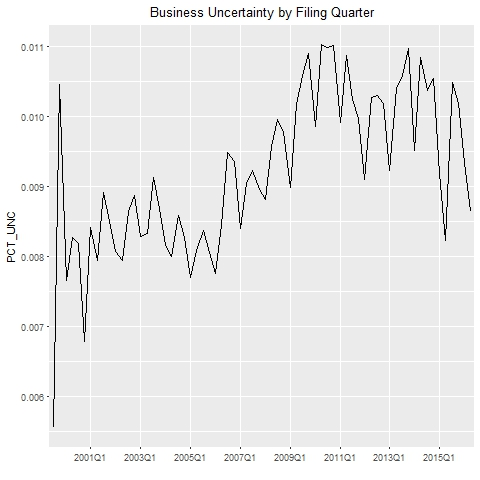
\includegraphics[width=6in, height=3in]{figures/bunc-by-quarter}
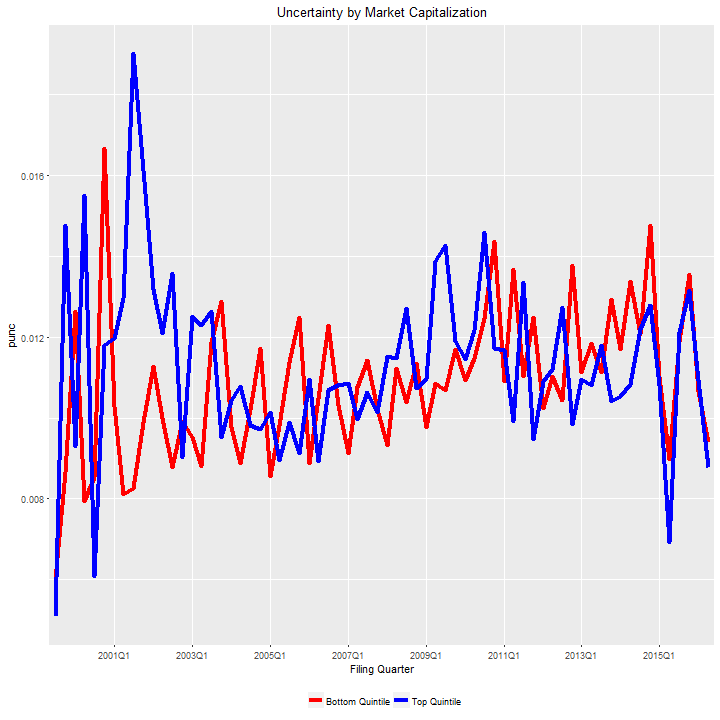
\includegraphics[width=6in, height=3in]{figures/bunc-by-mve}
\captionsetup{justification=centering, width=.95\textwidth} 
\caption{\footnotesize (Top panel) Time series trends of uncertainty} \label{bunc-figures}
\end{figure} 
\newpage
% TS and XS Total Assets
\begin{figure}[H] 
\centering
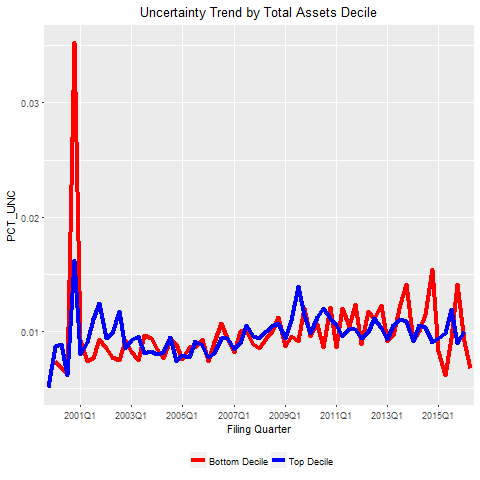
\includegraphics[width=3in, height=3in]{figures/punc-by-at-ts}
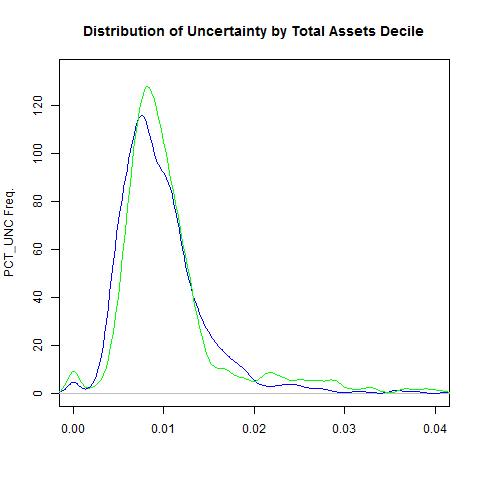
\includegraphics[width=3in, height=3in]{figures/punc-by-at-xs}
\captionsetup{justification=centering, width=.95\textwidth} 
\caption{\footnotesize Time series trends (left) and cross-sectional distribution (right) of uncertainty by total assets quintile.} \label{bunc-at}
\end{figure} 
% TS and XS Market-to-Book
\begin{figure}[H] 
\centering
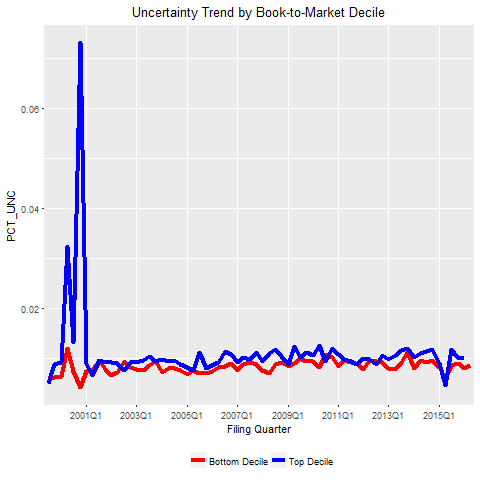
\includegraphics[width=3in, height=3in]{figures/punc-by-bm-ts}
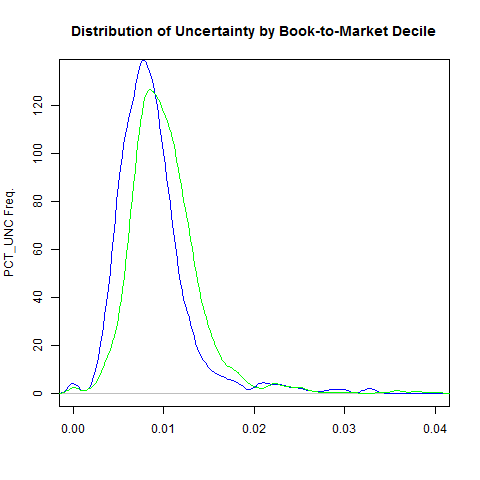
\includegraphics[width=3in, height=3in]{figures/punc-by-bm-xs}
\captionsetup{justification=centering, width=.95\textwidth} 
\caption{\footnotesize Time series trends (left) and cross-sectional distribution (right) of uncertainty by book-to-market quintile.} \label{bunc-bm}
\end{figure} 
\newpage
% TS and XS Tangibility
\begin{figure}[H] 
\centering
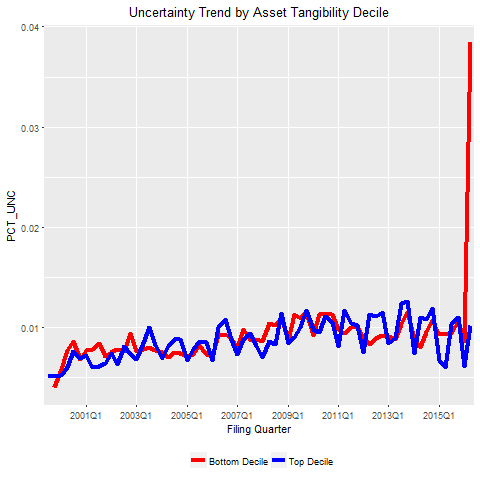
\includegraphics[width=3in, height=3in]{figures/punc-by-tang-ts}
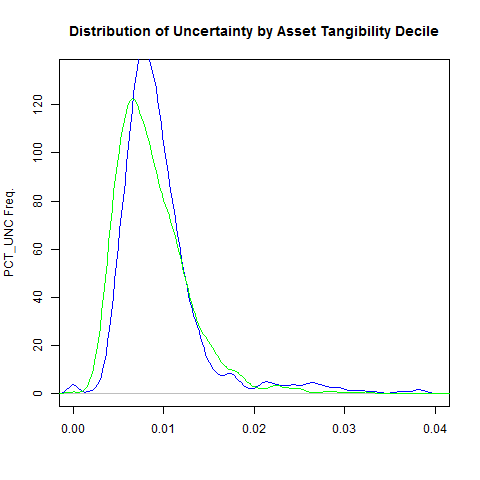
\includegraphics[width=3in, height=3in]{figures/punc-by-tang-xs}
\captionsetup{justification=centering, width=.95\textwidth} 
\caption{\footnotesize Time series trends (left) and cross-sectional distribution (right) of uncertainty by asset tangibility quintile.} \label{bunc-tang}
\end{figure} 
% TS and XS Forward PE
\begin{figure}[H] 
\centering
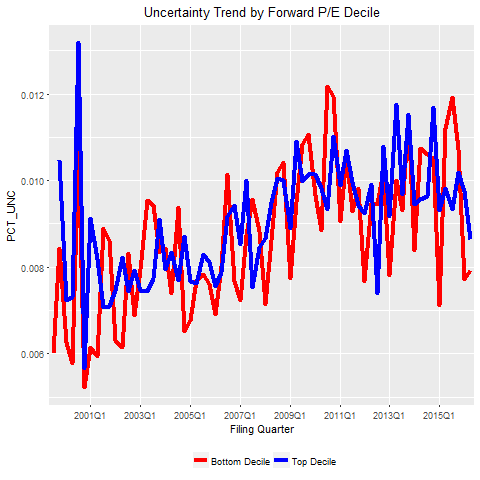
\includegraphics[width=3in, height=3in]{figures/punc-by-pefwd-ts}
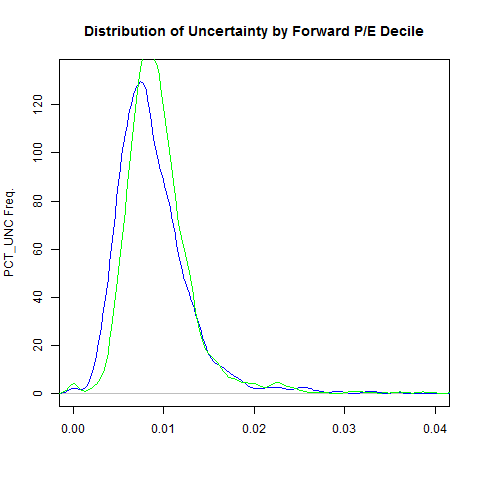
\includegraphics[width=3in, height=3in]{figures/punc-by-pefwd-xs}
\captionsetup{justification=centering, width=.95\textwidth} 
\caption{\footnotesize Time series trends (left) and cross-sectional distribution (right) of uncertainty by forward PE quintile.} \label{bunc-pefwd}
\end{figure} 
\newpage
% TS and XS Price
\begin{figure}[H] 
\centering
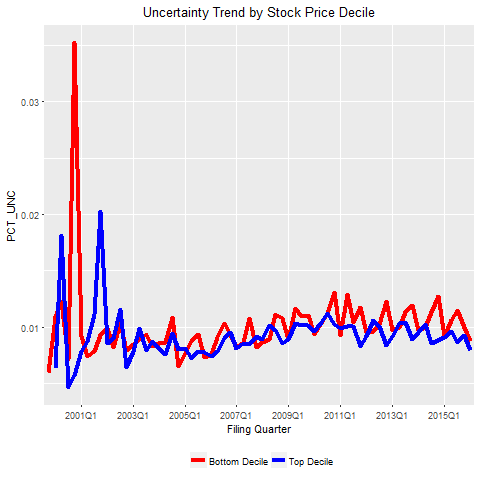
\includegraphics[width=3in, height=3in]{figures/punc-by-price-ts}
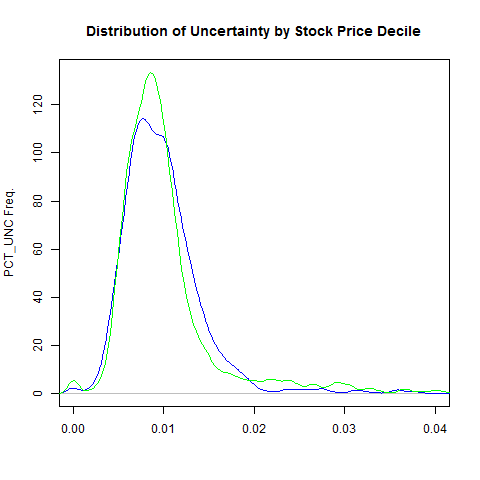
\includegraphics[width=3in, height=3in]{figures/punc-by-price-xs}
\captionsetup{justification=centering, width=.95\textwidth} 
\caption{\footnotesize Time series trends (left) and cross-sectional distribution (right) of uncertainty by stock price quintile.} \label{bunc-price}
\end{figure} 
% TS and XS Returns
\begin{figure}[H] 
\centering
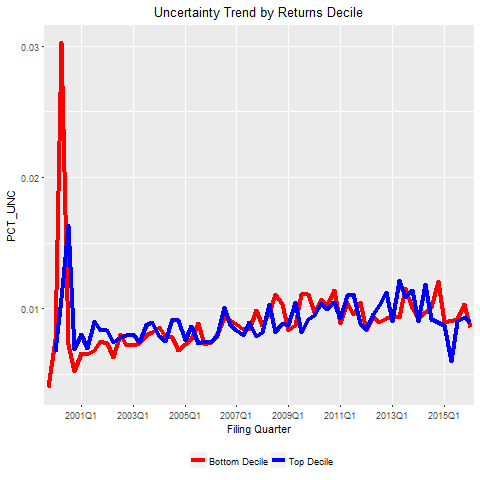
\includegraphics[width=3in, height=3in]{figures/punc-by-bhr-ts}
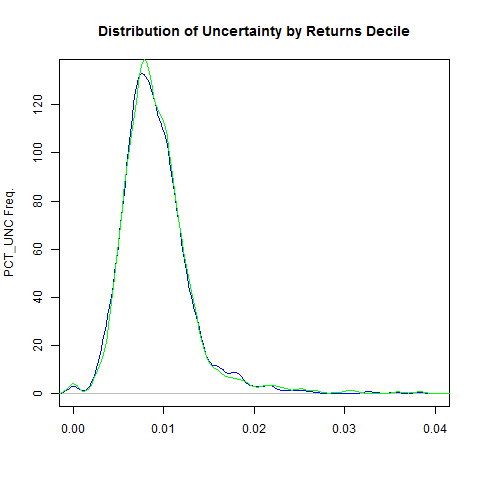
\includegraphics[width=3in, height=3in]{figures/punc-by-bhr-xs}
\captionsetup{justification=centering, width=.95\textwidth} 
\caption{\footnotesize Time series trends (left) and cross-sectional distribution (right) of uncertainty by stock returns quintile.} \label{bunc-bhr}
\end{figure} 
\newpage
% TS and XS Turnover
\begin{figure}[H] 
\centering
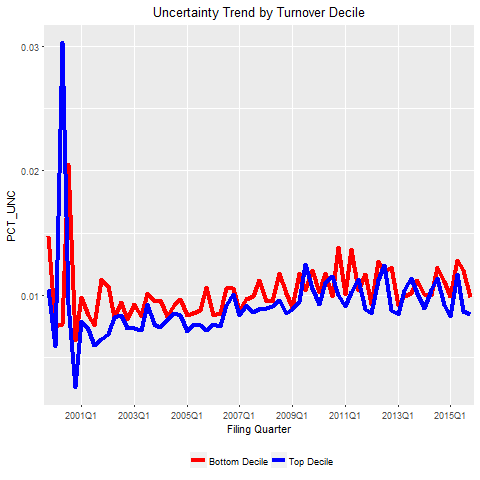
\includegraphics[width=3in, height=3in]{figures/punc-by-turn-ts}
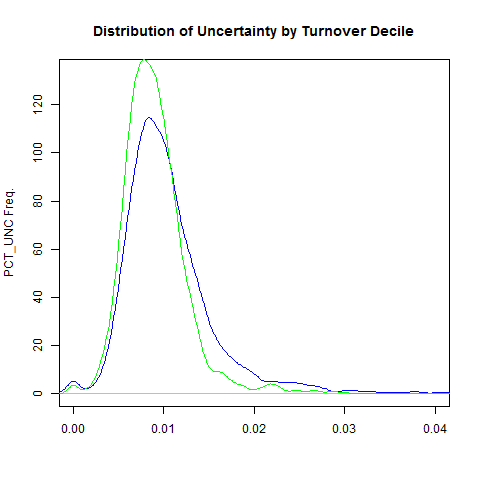
\includegraphics[width=3in, height=3in]{figures/punc-by-turn-xs}
\captionsetup{justification=centering, width=.95\textwidth} 
\caption{\footnotesize Time series trends (left) and cross-sectional distribution (right) of uncertainty by stock turnover quintile.} \label{bunc-turn}
\end{figure} 
\newpage
% TS and XS NANALYSTS
\begin{figure}[H] 
\centering
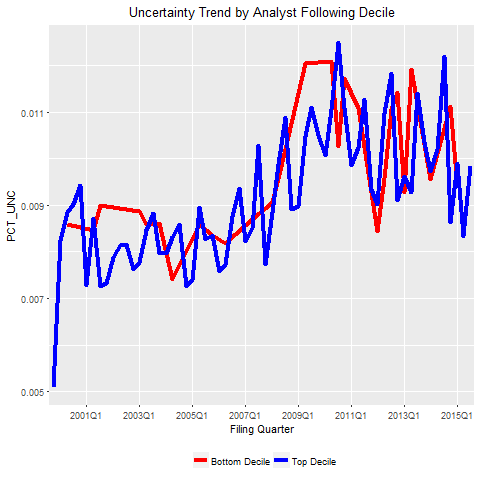
\includegraphics[width=3in, height=3in]{figures/punc-by-nanalysts-ts}
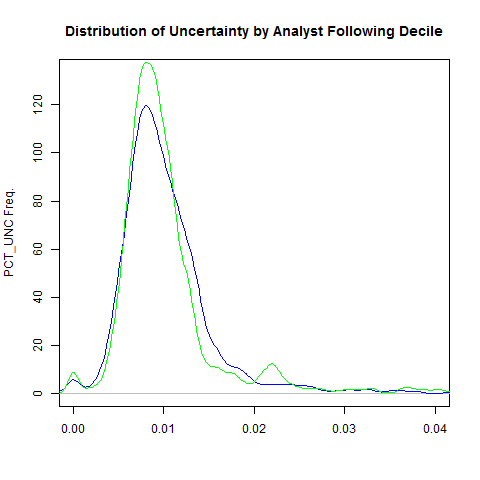
\includegraphics[width=3in, height=3in]{figures/punc-by-nanalysts-xs}
\captionsetup{justification=centering, width=.95\textwidth} 
\caption{\footnotesize Time series trends (left) and cross-sectional distribution (right) of uncertainty by analyst following quintile.} \label{bunc-nanalysts}
\end{figure} 
% TS and XS Analyst Dispersion
\begin{figure}[H] 
\centering
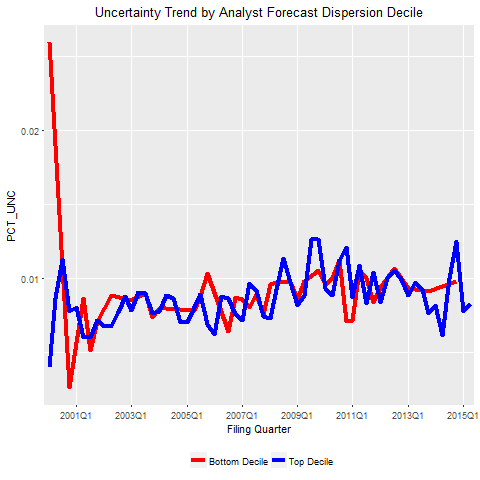
\includegraphics[width=3in, height=3in]{figures/punc-by-dispersion-ts}
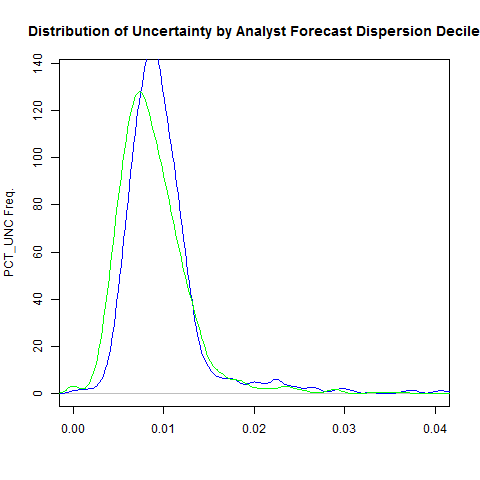
\includegraphics[width=3in, height=3in]{figures/punc-by-dispersion-xs}
\captionsetup{justification=centering, width=.95\textwidth} 
\caption{\footnotesize Time series trends (left) and cross-sectional distribution (right) of uncertainty by analyst forecast dispersion quintile.} \label{bunc-disp}
\end{figure} 
\newpage
%% Time series plots of aggregates
%%ROA
\begin{figure}[H] 
\centering
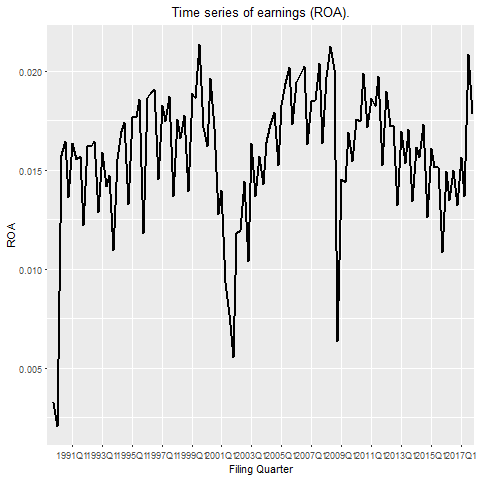
\includegraphics[width=5in, height=2.66in]{figures/roa-ts}
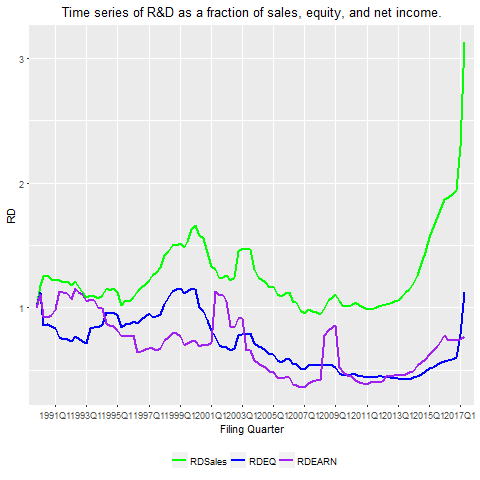
\includegraphics[width=5in, height=2.66in]{figures/rd-ts}
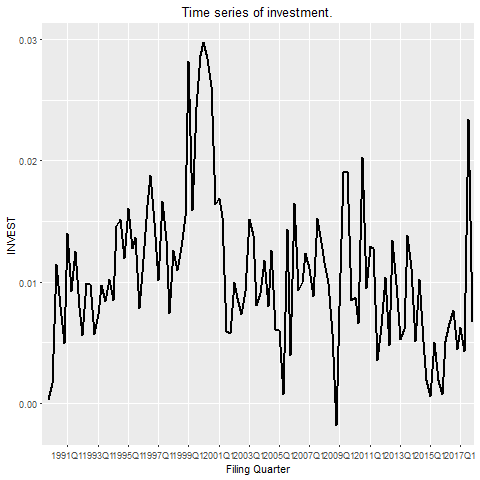
\includegraphics[width=5in, height=2.66in]{figures/invest-ts}
\captionsetup{justification=centering, width=.95\textwidth} 
\caption{\footnotesize Time series trends of Earnings, R\&D, and Investment} \label{ts-plots}
\end{figure} 
 \newpage 

%%ACF and PACF Plots: ROA
\begin{figure}[H] 
\centering
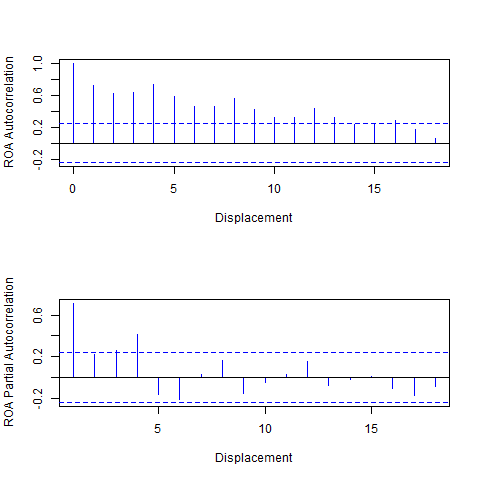
\includegraphics[width=5in, height=6in]{figures/roa-acf}
\captionsetup{justification=centering, width=.95\textwidth} 
\caption{\footnotesize Earnings (ROA) sample autocorrelation and partial autocorellation functions.} \label{roa-acf}
\end{figure} 
 \newpage 

%%ACF and PACF Plots: Investment
\begin{figure}[H] 
\centering
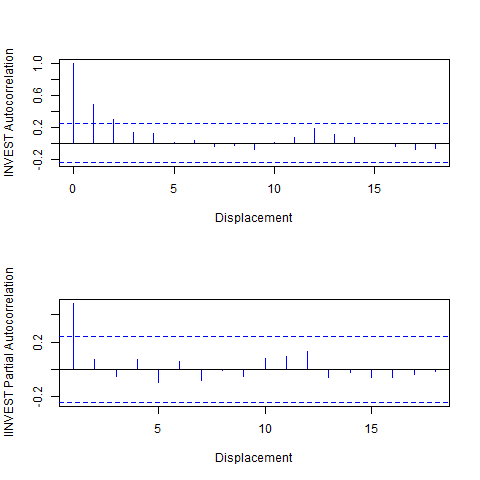
\includegraphics[width=5in, height=6in]{figures/invest-acf}
\captionsetup{justification=centering, width=.95\textwidth} 
\caption{\footnotesize Investment sample autocorrelation and partial autocorellation functions.} \label{invest-acf}
\end{figure} 
 \newpage 

%%ACF and PACF Plots: RD
\begin{figure}[H] 
\centering
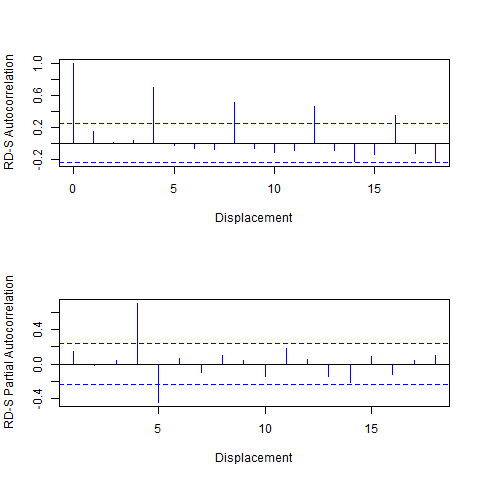
\includegraphics[width=5in, height=6in]{figures/rdsales-acf}
\captionsetup{justification=centering, width=.95\textwidth} 
\caption{\footnotesize R\&D sample autocorrelation and partial autocorellation functions.} \label{rd-acf}
\end{figure} 
 \newpage

%% VAR
\begin{figure}[H] 
\centering
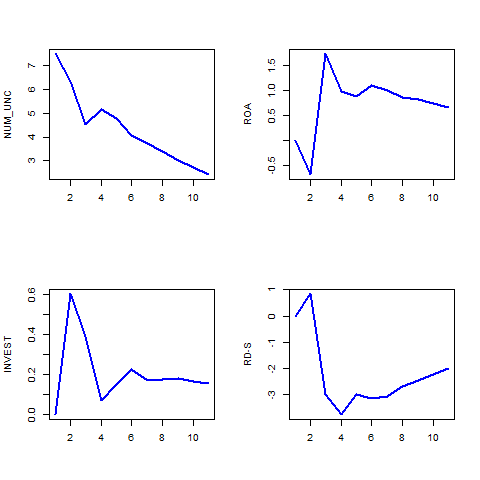
\includegraphics[width=6in, height=6in]{figures/nunc-irf-2}
\captionsetup{justification=centering, width=.95\textwidth} 
\caption{\footnotesize Impulse-Response Functions for $NUM\_UNC$.} \label{nunc-irf-2}
\end{figure} 
 \newpage
\begin{figure}[H] 
\centering
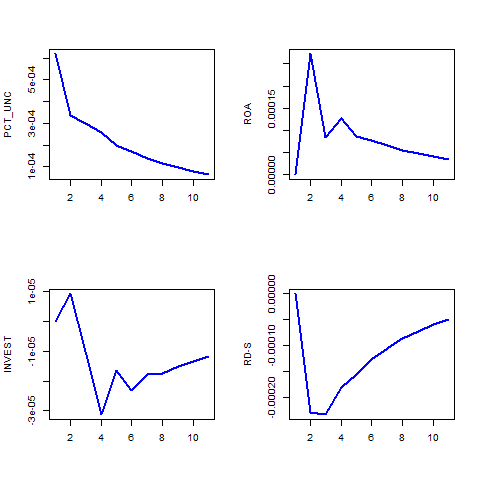
\includegraphics[width=6in, height=6in]{figures/punc-irf-2}
\captionsetup{justification=centering, width=.95\textwidth} 
\caption{\footnotesize Impulse-Response Functions for $PCT\_UNC$.} \label{punc-irf-2}
\end{figure} 
 \newpage
%% CCF Plots
\begin{figure}[H] 
\centering
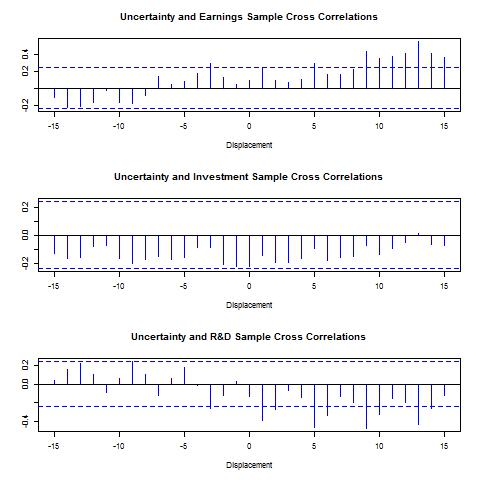
\includegraphics[width=6in, height=8in]{figures/ccf}
\captionsetup{justification=centering, width=.95\textwidth} 
\caption{\footnotesize Sample Cross-Correlation Plots} \label{ccf-plots}
\end{figure} 

\end{document}
